\chapter{Hierarchical Program Structures}

{
	\noindent
	\scshape\hfill\scriptsize Ole-Johan Dahl and C. A. R. Hoare\hfill
}
\renewcommand{\leftmark}{\normalfont\scriptsize\hfill OLE-JOHAN DAHL AND C. A. R. HOARE\hfill}

\section{Introduction}

In this monograph we shall explore certain ways of program structuring and point out their relationship to concept modeling.

We shall make use of the programming language SIMULA 67 with particular emphasis on structuring mechanisms. SIMULA 67 is based on ALGOL 60 and contains a slightly restricted and modified version of ALGOL 60 as a subset. Additional language features are motivated and explained informally when introduced. The student should have a good knowledge of ALGOL 60 and preferably be acquainted with list processing techniques.

For a full exposition of the SIMULA language we refer to the ``Simula 67 Common Base Language'' [\hyperref[ref:2]{2}]. Some of the linguistic mechanisms introduced in the monograph are currently outside the ``Common Base''\footnote{The Simula 67 language was originally designed at the Norwegian Computing Center, Oslo. The Common Base defines those language features which are common to all implementations. The Common Base is continually being maintained and revised by the ``Simula Standards Group'', each of whose members represents an organization responsible for an implementation. 8 organizations are currently represented on the SSG. (Summer 1971).}.

The monograph is an extension and reworking of a series of lectures given by Dahl at the NATO Summer School on Programming, Marktoberdorf 1970. Some of the added material is based on programming examples that have occurred elsewhere [\hyperref[ref:3]{3}, \hyperref[ref:4]{4}, \hyperref[ref:5]{5}].

\section{Preliminaries}

\subsection{Basic concepts}

Our subject matter as programmers is a special class of dynamic system, which we call computing processes or data processes. A programming language provides us with basic concepts and composition rules for constructing and analyzing computing processes.

The following are some of the basic concepts provided by ALGOL 60.

\begin{enumerate}[wide, nosep, label=(\arabic*)]
	\item A \textit{type} is a class of \textit{values}. Associated with each type there are a number of operations which apply to such values, e.g. arithmetic operations and relations for values of type \textbf{integer}.
	\item A \textit{variable} is a class of values of a given type ordered in a time sequence. The associated operations are accessing and assigning its current value. Both can be understood as \textit{copying} operations.
	\item An \textit{array} is a class of variables ordered in a spatial pattern. Associated is the operation of \textit{subscripting}.
\end{enumerate}

Notice that each of the concepts includes a data structure as well as one or more associated operations.

As another example consider machine level programming. The fundamental data structure is a bit string, which is not itself a very meaningful thing. However, combined with an appropriate sensing mechanism it has the significance of a sequence of Boolean values. In connection with a binary adder the bit string has the meaning of a number in some range, each bit being a digit in the base two number system. An output channel coupled to a line printer turns the bit string into a sequence of characters, and so forth. Thus the meaning of the data structure critically depends on the kind of operations associated with it.

On the other hand, no data process is conceivable which does not involve some data. In short, data and operations on data seem to be so closely connected in our minds, that it takes elements of both kinds to make up any concept useful for understanding computing processes.

\subsection{Higher level concepts}

As the result of the large capacity of computing instruments, we have to deal with computing processes of such complexity that they can hardly be constructed and understood in terms of basic general purpose concepts. The limit is set by the nature of our own intellect: precise thinking is possible only in terms of a \textit{small} number of elements at a time.

The only efficient way to deal with complicated systems is in a hierarchical fashion. The dynamic system is constructed and understood in terms of high level concepts, which are in turn constructed and understood in terms of lower level concepts, and so forth. This must be reflected in the \textit{structure} of the program which defines the dynamic system; in some way or another the higher level concepts will correspond to program components.

The construction of concepts suitable in a given situation is a creative process which often requires insights obtained at later stages of the system construction. Therefore, as programmers are painfully aware, any software project tends to be a complicated iterative process involving reconstruction and revision at each stage.

Each concept necessarily concerns a limited aspect of the system and
should correspond to a piece of program obtained by \textit{decomposition} of the total program. Good decomposition means that each component may be programmed independently and revised with no, or reasonably few, implications for the rest of the system. Thereby the total iteration process may be speeded up.

Any useful concept has some degree of generality, i.e. it is a class of
specialized instances. In other words one tries to group phenomena occurring in a dynamic system into \textit{classes} of phenomena and to describe each class by a single piece of program.

As an obvious example consider the arithmetic operations involved in a matrix multiplication. They may all be classified as dynamic instances (executions) of the single statement
$$
C[i, j] \coloneq C[i,j] + A[i, k] \times B[k, j];
$$

\noindent
provided that the matrix coefficients are classified as elements of two-dimensional arrays $A$, $B$, and $C$, and that the variables $i$, $j$, and $k$ are given values according to a certain pattern.

The above statement is not sufficiently well decomposed to be thought of as a ``concept''. The procedure declaration below, however, defines in a concise way the concept of matrix multiplication.

It is important that a concept may be classified as a \textit{syntactic category} (e.g. $\langle$block$\rangle$, $\langle$procedure$\rangle$) in a general language framework. Structured thought in terms of given concepts implies the construction of sentences, where the concepts have syntactic and semantic relationships to one another. The procedure below is related to other program components through calling sequences (procedure statements).

\quad \textbf{procedure} matmult$(A,\ B,\ C,\ m,\ n,\ p)$;

\quad \quad \textbf{array} $A$, $B$, $C$; \textbf{integer} $m$, $n$, $p$;

\quad \textbf{begin integer} $i$, $j$, $k$;

\quad \quad \textbf{for} $i\coloneq 1$ \textbf{step} 1 \textbf{until} $m$ \textbf{do}

\quad \quad \textbf{for} $j\coloneq 1$ \textbf{step} 1 \textbf{until} $n$ \textbf{do}

\quad \quad \textbf{begin} $C[i, j]\coloneq 0$;

\quad \quad \quad \textbf{for} $k\coloneq 1$ \textbf{step} 1 \textbf{until} $p$ \textbf{do}

\quad \quad \quad \quad $C[i, j]\coloneq C[i, j] + A[i, k] \times B[k, i]$

\quad \quad \textbf{end}

\quad \textbf{end};

The parameter mechanism of procedures in SIMULA deviates somewhat from that of ALGOL 60. The default transmission mode is by value for ordinary simple $\langle$type$\rangle$ parameters, and by ``reference'' for parameters of other kinds. This deviation is introduced for various pragmatic reasons, one of them being the compatibility with class declarations (cf. \ref{sec:frequency-histogram}). Thus, in the above procedure the parameters $i$, $j$, and $k$ are called by value, $A$, $B$, and $C$ by reference.

\subsection{Blocks and block instances}

One of the most powerful mechanisms for program structuring in ALGOL 60 is the block and procedure concept. It has the following useful properties from the standpoint of concept modeling.

\begin{enumerate}[wide, nosep, label=(\arabic*)]
	\item \textit{Duality}. A block head and block tail together define an entity which \textit{has properties} and \textit{performs actions}. Furthermore the properties may include a data structure as well as associated operators (local procedures).
	
	\item \textit{Decomposition}. A block where only local quantities are referenced is a completely self-contained program component, which will function as specified in any context. Through a procedure heading a block (procedure) instance may interact with a calling sequence. Procedures which reference or change non-local variables represent a partial decomposition of the total task, which is useful for direct interaction with the program environment.

	\item \textit{Class of instances}. In ALGOL 60 a sharp distinction is made between a block, which is a piece of program text, and a dynamic block instance, which is (a component of) a computing process. An immediate and useful consequence is that a block may be identified with the \textit{class} of its potential activation. (Strictly speaking a ``block'' in this context means either the outermost block or a block immediately enclosed by a dynamic block instance.) Through the recursion mechanism of ALGOL 60 different instances of the same block may co-exist in a computing process at the same time.

	\item \textit{Language element}. A block is itself a statement, which is a syntactic category of the language. Furthermore, through the procedure mechanism, reference to a block may be dissociated from its defining text.
\end{enumerate}

Referring back to our earlier discussion it appears that the ALGOL block mechanism has all the properties required of a concept modeling mechanism. On closer inspection, however, it turns out that the composition rules and interaction mechanisms provided place certain restrictions on the range of concepts to be formulated.

In ALGOL 60, the rules of the language have been carefully designed to ensure that the lifetimes of block instances are nested, in the sense that those instances that are latest activated are the first to go out of existence. It is this feature that permits an ALGOL 60 implementation to take advantage of a stack as a method of dynamic storage allocation and relinquishment. But it has the disadvantage that a program which creates a new block instance can never interact with it as an object which exists and has attributes, since it has disappeared by the time the calling program regains control. Thus the calling program can observe only the results of the actions of the procedures it calls. Consequently, the operational aspects of a block are overemphasized; and algorithms (for example, matrix multiplication) are the only concepts that can be modeled.

In SIMULA 67, a block instance is permitted to outlive its calling statement, and to remain in existence for as long as the program needs to refer to it. It may even outlive the block instance that called it into existence. As a consequence, it is no longer possible to administer storage allocation as a simple stack; a general garbage-collector, including a scan-mark operation, is required to detect and reclaim those areas of store (local workspace of block instances) which can no longer be referenced by the running program. The reason for accepting this extra complexity is that it permits a wider range of concepts to be conveniently expressed. In particular, it clarifies the relationship between data and the operations which may be performed upon it, in a way which is awkward or impossible in ALGOL 60.

\section[Object classes]{Object Classes}

A procedure which is capable of giving rise to block instances which survive its call will be known as a class; and the instances will be known as objects of that class. A class may be declared, with or without parameters, in exactly the same way as a procedure: 

\quad $\langle$class declaration$\rangle ::=$ \textbf{class} $\langle$class identifier$\rangle$

\tabto*{11.6em}$\langle$formal parameter part$\rangle$; $\langle$specification part$\rangle$;

\tabto*{11.6em}$\langle$class body$\rangle$

\quad $\langle$class body$\rangle ::= \langle$statement$\rangle$

Any variables or procedures declared local to the class body are called \textit{attributes} of that class; and so are the formal parameters, whether called by
value or called by reference. If the class body is not a block, it is regarded as if it were surrounded by block brackets \textbf{begin}\dots\textbf{end}.

A call of a class generates a new object of that class. The initial values of those of its attributes corresponding to formal parameters are specified in the actual parameter part of the generator. A generator always appears as a function designator, returning as its value a \textit{reference} to the newly generated object:

\quad $\langle$object generator$\rangle ::=$ \textbf{new} $\langle$class identifier$\rangle$

\tabto*{11.6em}$\langle$actual parameter part$\rangle$

In order to be able to refer again to a generated object, it is necessary to store the reference to it in a variable. Variables used for this purpose should be declared as of \textit{reference} type; and the declaration should also be \textit{qualified} by stating the class of objects to which that variable will refer.

\quad $\langle$reference variable declaration$\rangle ::=$ \textbf{ref} $(\langle $qualification$\rangle) \langle$identifier list$\rangle$

\quad $\langle$qualification$\rangle ::= \langle$class identifier$\rangle$

\noindent
The notation \textbf{ref} $(\langle$qualification$\rangle)$ may also be used to declare reference arrays, procedures, and parameters. An analogous mechanism for ``record handling'' was first proposed by Hoare [\hyperref[ref:6]{6}].

There is a neutral reference value \textbf{none} which does not refer to any object; and this is automatically assigned as initial value to every reference variable.

Reference values may be assigned, and tested for equality or inequality; but in SIMULA these operations are given special symbols, in order to emphasize the fact that they operate on references to objects, and not upon the current values contained in those objects.

\noindent
Thus:

\quad $:-$\tabto*{5.6em} denotes reference assignment

\quad $=\ =$\tabto*{5.6em} denotes reference equality

\quad $=/=$\tabto*{5.6em} denotes reference inequality.

\noindent
Reference values may also be passed as parameters, and they may be returned as the result of a function designator. A special example of such a function designator is of course the object generator which brings the object into existence, and passes back a reference to it as result.

\noindent
\textit{Example}:

\quad \textbf{class} $C(\dots)$; \dots class body for $C\dots$;

\quad \textbf{ref} $(C)X$;

\qquad \dots

\qquad \textbf{if} $X ==$ \textbf{none then} $X$: $-$ \textbf{new} $C(\dots)$;

The attributes of any object may be inspected or changed by the technique of \textit{remote identification}. If $X$ is a reference variable qualified by class $C$, and $A$ is an attribute identifier (i.e. local quantity) of that class, then $X.\,A$ refers to the attribute $A$ of the object currently referenced by $X$. If $X$ has the value \textbf{none}, the remote access is erroneous. If $A$ is a variable attribute, $X.\,A$ may appear to the left of an assignment, as an actual parameter, or in an expression. If $A$ is a procedure attribute, $X.\,A$ may appear as an actual parameter, or as a procedure statement or function designator, in which case it will be immediately followed by an actual parameter part. In short, a remote identifier $X.\,A$ may appear in any context in which an ordinary identifier may appear, except for a defining occurrence in a declaration.

In addition to reference variables, every reference parameter, function or expression has a qualification associated with it. In every assignment to a reference variable, it is possible to check that the assignment is valid, by comparing the qualifications of the left hand and right hand sides. SIMULA 67 has been designed to ensure that this check can be carried out wholly at compile time, thus avoiding the inefficiency of run-time checking, and the inconvenience of run-time error. Furthermore all remote identifiers can be checked at compile time to ensure that the combination of reference variable and attribute identifier is valid, so that the only error that has to be detected at run-time is when the reference variable has the value \textbf{none}.

The following sections provide examples of concepts modeled by means of class declarations.


\subsection{Frequency histogram}
\label{sec:frequency-histogram}

A frequency histogram of a real random variable with respect to given disjoint intervals can be represented by a table of integers $T_0, T_1, \dots, T_n$, where $T_i$ is the number of observations falling in the $i$th interval. A sequence of increasing numbers $X_1, X_2, \dots, X_n$ partitions the real axis into the following $n + 1$ intervals:
$$
\langle -\infty, X_1\rangle, (X_1, X_2\rangle, \dots, (X_n, \infty\rangle.
$$

\noindent
The $i$th relative frequency $(i = 0, 1, \dots, n)$ is equal to $T_i / N$, where $N$ is the total number of observations tabulated in the histogram.

We wish to represent the concept of a histogram as a self-contained piece of program, which can be incorporated in any subsequently written program which requires it. In a realistic program, it will be necessary to maintain several histograms to tabulate different random variables; for example, it may be necessary to record not only random lengths, but also random weights and random heights, and this will require three separate histograms, existing simultaneously with each other and with the main program which has generated them and which is using them. Furthermore, the numbers of the intervals and the partitioning values between them may be different in each case. This suggests that the histogram should be declared as a \textit{class}, with two parameters:

\quad \textbf{class} histogram$(X, n)$; \textbf{array} $X$; \textbf{integer} $n$;

\noindent
where $X$ is a real array of $n$ elements specifying the boundaries of the partitions. The main program will use this class in the following way:

\quad \textbf{begin ref} $($histogram$)$ heights, weights, lengths;

\quad \quad \textbf{real array} $A[1:7]$, $B[1:12]$;

\quad \quad \dots initialise $A$, $B$\dots;

\quad \quad heights: $-$ \textbf{new} histogram$(A,\ 7)$;

\quad \quad weights: $-$ \textbf{new} histogram$(B,\ 12)$;

\quad \quad lengths: $-$ \textbf{new} histogram$(A,\ 7)$;

\quad \quad \dots rest of program\dots

\quad \textbf{end}

In the rest of the program, the three histograms may be referred to by the names of the three reference variables. In order to record each new observation (say $h$ or $w$) in the appropriate histogram, the program will contain the corresponding calls on a procedure tabulate:

\quad weights.tabulate$(w);$

\quad heights.tabulate$(h);$

\noindent
The procedure ``tabulate'' must therefore be an attribute of the histogram class. Another attribute of the class must be the array $T$ which counts the number of observations in each interval; and also a variable $N$ to count the total number of observations recorded so far. Finally, a function frequency$(i)$ is required so that the relative frequency of observations in the $i$th interval may be read out. The only action required of the class body is to initialize these variables.

The declaration of the histogram class may be given:

\quad \textbf{class} histogram$(X,\ n)$; \textbf{array} $X$; \textbf{integer} $n$;

\quad \quad \textbf{begin integer} $N$; \textbf{integer array} $T[0:n]$;

\quad \quad \quad \textbf{procedure} tabulate$(Y)$; \textbf{real} $Y$;

\quad \quad \quad \quad \textbf{begin integer} $i$; $i\coloneq 0$;

\quad \quad \quad \quad \quad \textbf{while} (\textbf{if} $i < n$ \textbf{then} $Y < X[i + 1]$ \textbf{else false}$)$

\quad \quad \quad \quad \quad \quad \textbf{do} $i\coloneq i + 1$;

\quad \quad \quad \quad \quad $T[i] \coloneq T[i] + 1; N\coloneq N + 1$

\quad \quad \quad \quad \textbf{end} of tabulate;

\quad \quad \quad \textbf{real procedure} frequency$(i)$; \textbf{integer} $i$;

\quad \quad \quad \quad frequency $\coloneq T[i]/N$;

\quad \quad \quad \textbf{integer} i;

\quad \quad \quad \textbf{for} $i\coloneq 0$ \textbf{step} 1 \textbf{until} $n$ \textbf{do} $T[i]\coloneq 0;\ N\coloneq 0$

\quad \textbf{end} of histogram;

\textit{Note}. (1) In SIMULA 67, all simple parameters of a class or a procedure are called by value, even if the value parts are omitted. Arrays and other parameters are called by name.

(2) In SIMULA 67 all variables are automatically initialized on declaration to neutral values, \textbf{false} for Booleans, 0 for numbers, \textbf{none} for references. Thus in the examples given above the statements $i\coloneq 0,\ N\coloneq 0$, and the loop initializing $T$ could have been omitted.

It seems reasonable to claim that this piece of program adequately represents the concept of a histogram, in that it expresses the close relationship between the data items $X$, $n$, $T$ and $N$, and the operation of tabulation which
is to be performed on them. It would be possible, of course, to write the
operation in ALGOL 60 as a separate procedure with many parameters:

\quad \textbf{procedure} tabulate$(X,\ n,\ T,\ N,\ y)$;

\noindent
which records observation $y$ in the histogram $T$ in accordance with partitions defined by $X$, and also increments $N$. But this would be an artificial separation
of the operational aspect of the histogram from the data storage aspect; and the failure in adequately representing the concept is evidenced by the complexity of the specification of the procedure and the awkwardness of its use. 

It is worth while to explain the effect of creating a new object of class histogram by means of the statement

\quad weights: $-$ \textbf{new} histogram$(B,\ 12)$.

\noindent
First, a new object is created, consisting of the variables brought into existence by execution of the declarations for $T$, $N$, $i$, and the parameters $X$ and $n$, which are initialized to $B$ and 12 respectively. The body of the class declaration is now executed to initialize the other variables. On exit from the body, the variables are \textit{not} deallocated. Rather a reference (pointer, address) to them is passed back and assigned to the variable ``weights''. It is convenient to think of an object as a complete textual copy of the class body (including the specification part), in which the parameters and local variables and arrays correspond to actual storage locations. Thus an object may well contain local procedure (and even class $-$) declarations, as well as executable statements.

Subsequently, on execution of the procedure call weights. tabulate($w$), it is the tabulate procedure local to the object referenced by ``weights'' that is actually executed, and causes updating of the local attributes $T$ and $N$ of that object and no other.

\subsection{Gauss-integration}

A definite integral may be approximated by an ``$n$-point Gauss formula'', which is a weighted sum of $n$ function values computed at certain points in the integration interval.
$$
\int_a^b f(x)\text{d}x \approx \sum_{i = 1}^n w_i f(x_i)
$$

\noindent
The weights and abscissa values are chosen such as to give an exact result for the integral of any polynomial of degree less than $2n$. By a suitable transformation we find
$$
w_i = (b - a)W_i \quad\text{and}\quad x_i = a + (b - a)X_i,
$$

\noindent
where $W_i$ and $X_i(i = 1, 2, \dots, n)$ only depend on $n$, and not on $a$ or $b$. The idea of Gauss-integration is expressed in the following partly informal class declaration.

\quad \textbf{class} Gauss$(n)$; \textbf{integer} $n$;

\quad \textbf{begin array} $W$, $X[1:n]$;

\quad \quad \textbf{real procedure} integral$(f,\ a,\ b)$;

\quad \quad \textbf{real procedure} $f$; \textbf{real} $a$, $b$;

\quad \quad integral $\coloneq \sum_{i=1}^n W[i] \times f(a + (b - a)\times X[i])\times (b- a)$;

\quad \quad compute $W[1], \dots, W[n], X[1], \dots, X[n]$ as

\quad \quad functions of $n$

\quad \textbf{end} of Gauss;

\quad \dots

\quad \textbf{ref} $($Gauss$)$ G5, G7;

\quad \dots

\quad G5: $-$ \textbf{new} Gauss$(5)$; G7: $-$ \textbf{new} Gauss$(7)$;

\quad \dots

\quad G5.integral$(F,\ A,\ B)$ \dots G7.integral$(F,\ A,\ B)$\dots

\noindent
\textit{Comments}. The variables G5 and G7 refer to the concepts ``5-point'' and ``7-point Gauss-integration''. Each of them is a \textit{specialized instance} of the
more general concept of ``$n$-point Gauss-integration'', represented by the class.

A Gauss object computes once and for all the values of its local array elements, after which control returns to the $\langle$object generator$\rangle$. The procedure ``integral'' is intended for repeated use from outside the object.

The example indicates that the \textit{own}-concept of ALGOL is superfluous in this framework.

\section{Coroutines}

In ALGOL 60, a most powerful method of combining two pieces of program to accomplish some task is to declare one of them as a procedure, and to invoke it (possibly repeatedly) from within the other. However, in some cases the relationship between the two pieces of program is not fairly represented by this form of master$/$subordinate relationship; and it is better to regard them as \textit{coroutines} operating in some sense at the same level.

A simple example of coroutine structuring is provided by a games-playing program, which calculates its own move and outputs it to its opponent, inputs the opponent's response, computes its next move, and so on until the game is complete. Suppose now that two different programs have been constructed to play the same game, and it is desired to see which of them is the stronger player. The complete program to play the game is very naturally structured from its two component players, but the structuring method is that of the coroutine rather than the subroutine.

Another example of coroutine structuring is provided in a two-pass compiler for a programming language. The first pass normally outputs a long sequence of messages which are subsequently input by the second pass. However, if sufficient main storage is available to accommodate the program for both passes simultaneously, it is possible to arrange for the whole translation to be carried out apparently in a single pass, where the sequence of messages is transmitted \textit{piecewise} from the first pass to the second pass. First, the second pass is executed until it reaches its first request for an input message. The first pass program is then executed until it produces its first output message. The message is then handed over to the second pass, and the process is repeated until the second pass is complete. In some circumstances it might be possible to restructure one of the passes as a subroutine to the other; but since the choice would be arbitrary, it is better to regard the two programs as coroutines.

This case may be distinguished from the games-playing example in that the flow of information is in one direction only, from the first pass program which ``produces'' it to the second pass program which ``consumes'' it. This suggests that a single coroutine may profitably be regarded as a complete selfcontained program whose input and output instructions have been replaced by calls upon other coroutines to produce and consume the data. Each time a coroutine passes control to another coroutine for this purpose, it will expect to resume at the next following instruction. The instruction which causes transfer of control to another coroutine is known as

\quad resume$(X)$

\noindent
where $X$ refers to the coroutine being resumed.

In SIMULA, a coroutine is represented by an object of some class, cooperating by means of resume instructions with objects of the same or another class, which are named by means of reference variables. The communication of information may be accomplished in variables either global to all the objects or local to one of them; a producing coroutine assigns values to these variables, and the consuming coroutine accesses them. In the case of two-way communication, both coroutines may update the same global variables in turn.

When an object is first generated, it has a subordinate, procedurelike relationship to the block instance which generated it. This is evidenced by the fact that control automatically returns to the generator upon passage through the end of the object. The object does not in general know the identity of its generating block instance; it cannot therefore use a resume instruction to achieve the effect of a coroutine exit. A special, parameterless ``detach''' instruction is therefore provided by which a generated object can return control to the generator. The generator may then resume the detached object at the point following its (most recently executed) detach instruction by the
statement

\quad call$(X)$

\noindent
where $X$ is a reference to the detached object. Now the object is again in a subordinate position, with respect to the caller, and has an obligation to return to it either by a detach instruction or by going through its own \textbf{end}.

Thus a main program may establish a coroutine relationship with an object that it has generated, using the call$/$detach mechanism instead of the more symmetric resume$/$resume mechanism. In this case, the generated object remains subordinate to the main program, and for this reason is sometimes known as a \textit{semicoroutine}. But a semicoroutine may also be a full coroutine with respect to a group of other generated objects, with which it communicates by means of resume statements. In this case, if any of the group issues a detach, control returns to the master program which originally called a particular member of the group. Thus a coroutine issuing a resume statement imposes on the resumed coroutine its own responsibility, eventually to pass control back to the original caller by means of a detach.

Let $X$ and $Y$ be objects, generated by a ``master program'' $M$. Assume that $M$ issues a call$(X)$, thereby invoking an ``active phase'' of $X$, terminated by a detach operation in $X$; and then issues a call$(Y)$, and so forth. In this way $M$ may act as a ``supervisor'' sequencing a pattern of active phases of $X$, $Y$, and other objects. Each object is a ``slave'', which responds with an active phase each time it is called for, whereas $M$ has the responsibility to define the large scale pattern of the entire computation.
\begin{center}
	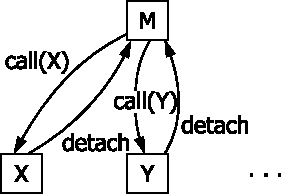
\includegraphics[width=.3\textwidth]{chap3/fig1}
\end{center}

\noindent
Alternatively the decision making may be ``decentralized'', allowing an object itself to determine its dynamic successor by a resume operation.

\begin{center}
	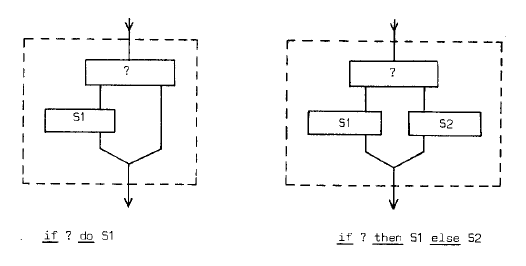
\includegraphics[width=.44\textwidth]{chap3/fig2}
\end{center}

\noindent
The operation resume$(Y)$, executed by $X$, combines an exit out of $X$ (by detach) and a subsequent call$(Y)$, thereby bypassing $M$. Obligation to return to $M$ is transferred to $Y$.

The history of a typical coroutine object may be summarized as follows:

\begin{enumerate}[wide, nosep, label=(\arabic*)]
	\item Upon generation, an object starts performing the operations of its class body, and is said to be \textit{operating} and \textit{attached} to (the block instance containing) the object generator which calls it into existence.
	\item The object issues a \textit{detach} statement which returns control to the point at which the object was generated. The object is then said to be detached, but not yet terminated. The detach statement leaves a mark in the body of the object specifying where its operations will be continued. This mark is positioned at the end of the detach statement most recently executed by that object.
	\item Control returns to the object on execution of either a call statement or a resume statement specifying that object by means of its reference parameter. It is then \textit{reattached} to the \textit{calling} block instance if called, or to the original caller if resumed. The object may then temporarily relinquish control again, either by a detach or by a resume, in which case it becomes detached again. 
	\item Alternatively, it may relinquish control finally by passing through its \textbf{end}, which has the same effect as a detach. But in this case it is said to be \textit{terminated}, and it may not be reactivated either by a call or a resume. However, it remains in existence as an item of data, which may be referenced by remote identification of its attributes, including procedure and function attributes, as in the case of the histogram.
\end{enumerate}

\textit{Note}. The detach operation represents a coroutine exit out of an \textit{object}, and is only available textually within objects, i.e. textually within class bodies. If issued in a sub block or in a procedure body, a detach instruction still represents an exit out of the (smallest) textually enclosing object. The same
is true for the resume instruction (which includes a coroutine exit). The call instruction is, however, available at any point in a program.

\subsection{Text transformation}

As an example of the cooperation of coroutines we take a problem posed by Conway [\hyperref[ref:7]{7}]. A text is to be read from cards and listed on a line printer. The cards each contain 80 characters, but the line printer prints 125 characters on each line. It is intended to pack as many characters as possible on each output line, marking the transition from one card to the next only by insertion of an extra space. In the text, any consecutive pair of asterisks is to be replaced by ``$\uparrow$''. The end of the text is marked by a special character known as ``end''.

We assume the existence of a coroutine ``incard'', which on each resumption will fill the array $C[1 : 80]$ with characters read from the next card in the card hopper, and pass the card through to the stacker. Also, we are given a coroutine ``lineout'', which on each resumption will print on the next line of paper the characters from the array $L[1 : 125]$, and then throw the line.

The task is carried out by three coroutines, which will be known by reference as:

\quad \textbf{ref} disassembler, squasher, assembler;

The disassembler inputs a card (through $C$) and outputs individual characters (through $c1$) to the squasher, after inserting a space between cards. The squasher performs the transformation on double asterisks, and outputs individual characters through $c2$ to the assembler. The assembler groups the characters into lines and outputs them; it also detects the ``end'' character and takes appropriate action.

The required class declarations are:

\quad \textbf{class} pass 1;

\quad \textbf{begin} detach;

\quad \quad \textbf{while true do}

\quad \quad \quad \textbf{begin integer} $i$; resume$($incard$)$;

\quad \quad \quad \quad \textbf{for} $i\coloneq 1$ \textbf{step} 1 \textbf{until} 80 \textbf{do}

\quad \quad \quad \quad \quad \textbf{begin} $c1\coloneq C[i]$; resume$($squasher$)$ \textbf{end};

\quad \quad \quad \quad $c1\coloneq$ blank; resume$($squasher$)$

\quad \quad \quad \textbf{end} infinite loop;

\quad \textbf{end} pass 1;

\quad \textbf{class} pass 2;

\quad \textbf{begin} detach;

\quad \quad \textbf{while true do}

\quad \quad \quad \textbf{begin if} $c1 =$ ``*'' \textbf{then}

\quad \quad \quad \quad \textbf{begin} resume$($disassembler$)$;

\quad \quad \quad \quad \quad \textbf{if} $c1 =$ ``*'' \textbf{then} c2: = ``$\uparrow$''

\quad \quad \quad \quad \quad \textbf{else begin} $c2 \coloneq$ ``*''; resume$($assembler$)$;

\quad \quad \quad \quad \quad \quad $c2\coloneq c1$

\quad \quad \quad \quad \quad \textbf{end};

\quad \quad \quad \quad \textbf{end}

\quad \quad \quad \textbf{else} $c2\coloneq c1$;

\quad \quad \quad resume (assembler); resume (disassembler)

\quad \textbf{end} infinite loop;

\quad \textbf{end} pass 2;

\quad \textbf{class} pass 3;

\quad \textbf{begin} detach;

\quad \quad \textbf{while true do}

\quad \quad \quad \textbf{begin integer} $i$;

\quad \quad \quad \quad \textbf{for} $i\coloneq 1$ \textbf{step} $1$ \textbf{until} 125 \textbf{do}

\quad \quad \quad \quad \quad \textbf{begin} $L[i] \coloneq c2$;

\quad \quad \quad \quad \quad \quad \textbf{if} $c2 =$ ``end'' \textbf{then}

\quad \quad \quad \quad \quad \quad \textbf{begin for} $i\coloneq i + 1$ \textbf{step} 1 \textbf{until} 125 \textbf{do}

\quad \quad \quad \quad \quad \quad \quad $L[i] \coloneq$ blank;

\quad \quad \quad \quad \quad \quad \quad resume$($lineout$)$;

\quad \quad \quad \quad \quad \quad \quad detach; \textbf{comment} back to main program;

\quad \quad \quad \quad \quad \quad \textbf{end}

\quad \quad \quad \quad \quad \quad \textbf{else} resume$($squasher$)$

\quad \quad \quad \quad \quad \quad \textbf{end} of this line;

\quad \quad \quad \quad resume$($lineout$)$

\quad \quad \quad \textbf{end} infinite loop

\quad \textbf{end} pass 3;

The main program generates one instance of each of the passes. Each pass immediately detaches itself from the main program. The system of coroutines is initiated by calling the disassembler. On detection of the end of the task, the assembler issues a detach instruction. Since the assembler obtained control (indirectly) by resume instructions from the disassembler, its detach has the same effect as it would have had if issued by the disassembler, and takes control back to the main program, which then immediately terminates.

The main program is:

\quad \textbf{begin} disassembler: $-$ \textbf{new} pass 1;

\quad \quad squasher: $-$ \textbf{new} pass 2;

\quad \quad assembler: $-$ \textbf{new} pass 3;

\quad \quad call$($disassembler$)$;

\quad \textbf{end}

The relationships between the five coroutines and the main program may be represented pictorially:
\begin{center}
	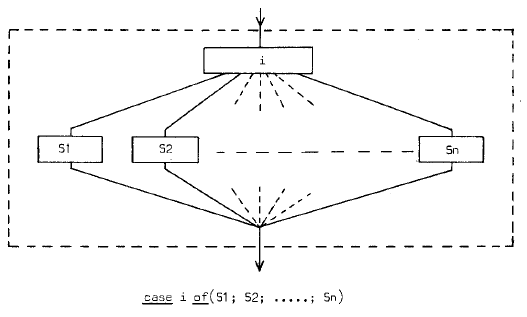
\includegraphics[width=.7\textwidth]{chap3/fig3}
\end{center}

\noindent
The horizontal arrows represent resume$/$resume relations. Their direction corresponds to the flow of information; and they are annotated by the name of the variable used to hold the communicated information.

In this example, it is intended that each class should only ever have one object in it; and therefore the full class$/$generation$/$reference mechanism is unnecessarily elaborate. The elaboration is inconvenient in that separate names have to be invented for the class and its unique object (e.g. pass 1 and disassembler). Furthermore, in the implementation it should be possible to take advantage of this special case to save both space and time. But SIMULA 67 provides no means of achieving this.

\subsection{Permutation generator}

We wish to define a class ``permuter'' representing the concept of permutations. An object of this class should be capable of generating all permutations of the integers between 1 and $n$, where $n$ is a parameter of the class. One of the attributes of the class will be an \textbf{integer array} $p[1:n]$, which is to be initialized to the value $(1, 2, \dots, n)$ (representing the identity permutation) when an object of the class is generated. Every subsequent call of the object
causes the array $p$ to take a new permutation as value. When all permutations are exhausted, an attribute 

\quad \textbf{Boolean} more;

\noindent
(initially true) will be assigned the value \textbf{false}, and the object will terminate.

A typical structure for a program which wishes to inspect all permutations of $N$ numbers will be:

\quad \textbf{ref} $($permuter$)P$;

\quad $P$: $-$ \textbf{new} permuter$(N)$;

\quad \textbf{while} $P$.more \textbf{do}

\quad \quad \textbf{begin}\dots inspect $P.p$\dots; call$(P)$ \textbf{end};

\noindent
The structure of the permuter class will be a semicoroutine, which issues a detach instruction after each updating of $p$:

\quad \textbf{class} permuter$(n)$; \textbf{integer} $n$;

\quad \quad \textbf{begin integer array} $p[1:n]$;

\quad \quad \quad \textbf{Boolean} more;

\quad \quad \quad \textbf{integer} $q$;

\quad \quad \quad \textbf{for} $q\coloneq 1$ \textbf{step} 1 \textbf{until} $n$ \textbf{do} $p[q]\coloneq q$;

\quad \quad \quad more $\coloneq$ \textbf{true};

\tabto*{3.3em} \dots generate all permutations of $p$,

\quad \quad \quad issuing a ``detach'' after each of them\dots;

\quad \quad \quad more $\coloneq$ \textbf{false}

\quad \quad \textbf{end}

It remains to find an algorithm to carry out all the permutations of $p[1]$, $p[2]$, \dots, $p[n]$, and restore them to their original state. This algorithm may be recursively structured. Let us assume that we know how to generate \textit{all} permutations of the numbers

\quad $p[1], p[2], \dots, p[k - 1],$

\noindent
and finally return these to their original state. This will be accomplished by a procedure call

\quad permute$(k - 1)$.

\noindent
Now all that need be done is to use this procedure to permute every \textit{combination} of $k - 1$ numbers from the original $k$ numbers. Thus there must be $k$ calls of permute$(k - 1)$, and on each call, exactly one of the $p[i]$ for $1 \leqslant i \leqslant k$ must be excluded from the operation. A good way of excluding it is to exchange its value with that of $p[k]$, which remains untouched by permute $(k - 1)$. In order to ensure that each of the $k$ values is excluded exactly once, we may take advantage of the assumption that the procedure returns the given sequence unchanged. In that case $p[k]$ will be assigned each value once if we first swap $p[1]$ and $p[k]$, then $p[2]$ and $p[k]$, \dots, and then $p[k - 1]$ and $p[k]$. Thus we are led to the following kernel:

\quad \textbf{integer} $i$;

\quad permute$(k - 1)$;

\quad \textbf{for} $i\coloneq 1$ \textbf{step} 1 \textbf{until} $k - 1$ \textbf{do}

\quad \quad \textbf{begin} swap$(p[i]$, $p[k])$; permute$(k - 1)$ \textbf{end};

\noindent
On the assumption that permute$(k - 1)$ leaves p unchanged, this kernel has the net effect of rotating the elements $p[1]$, $p[2]$, \dots, $p[k]$ one place cyclically to the right. This can be seen from the example:

\quad original state:\tabto*{12em}  1 2 3 4 5

\quad after swap$(p[1], p[5])$:\tabto*{12em} 5 2 3 4 1

\quad after swap$(p[2], p[5])$:\tabto*{12em}  5 1 3 4 2

\quad after swap$(p[3], p[5])$:\tabto*{12em}  5 1 2 4 3

\quad after swap$(p[4], p[5])$:\tabto*{12em}  5 1 2 3 4

\noindent
Since the overall effect of the operation must be to leave the array $p$ as it was before, the right rotation must be followed by a compensatory left rotation.

\quad $q\coloneq p[1];$

\quad \textbf{for} $i\coloneq 1$ \textbf{step} 1 \textbf{until} $k - 1$ \textbf{do} $p[i]\coloneq p[i + 1]$;

\quad $p[k]: = q$

\noindent
Finally it is necessary to determine an appropriate action for the case where $k = 1$. Recall that the purpose of the procedure is to 

\hangindent=1.9\parindent\quad ``generate all permutations of $k$ objects, issuing a detach command after each of them''.

\noindent
Since the only permutation of one number is that number itself, all that is necessary is to issue a single detach instruction.

The permute procedure must be written as an attribute of the permuter class, so that the detach which it issues relates to the relevant object. The whole class may now be declared:

\quad \textbf{class} permuter$(n)$; \textbf{integer} $n$;

\quad \textbf{begin integer array} $p[1:n]$; \textbf{integer} $q$; \textbf{Boolean} more;

\quad \quad \textbf{procedure} permute$(k)$; \textbf{integer} $k$;

\quad \quad \textbf{if} $k = 1$ \textbf{then} detach \textbf{else}

\quad \quad \textbf{begin integer} $i$; permute$(k - 1)$;

\quad \quad \quad \textbf{for} $i\coloneq 1$ \textbf{step} 1 \textbf{until} $k - 1$ \textbf{do}

\quad \quad \quad \textbf{begin} $q\coloneq p[i]$; $p[i]\coloneq p[k]$;

\quad \quad \quad \quad $p[k]\coloneq q$; permute$(k - 1)$

\quad \quad \quad \textbf{end};

\quad \quad \quad $q\coloneq p[1]$;

\quad \quad \quad \textbf{for} $i\coloneq 1$ \textbf{step} 1 \textbf{until} $k - 1$ \textbf{do} $p[i] \coloneq p[i + 1]$;

\quad \quad \quad $p[k]\coloneq q$

\quad \quad \textbf{end} of permute;

\quad \quad \textbf{for} $q\coloneq 1$ \textbf{step} 1 \textbf{until} $n$ \textbf{do} $p[q] \coloneq q$;

\quad \quad \quad more $\coloneq$ \textbf{true}; permute$(n)$; more $\coloneq$ \textbf{false}

\quad \textbf{end} of permuter;

\textit{Note}. The detach issued by a permute procedure instance is \textit{not} an exit out of the procedure instance, and does not return control to the call of the procedure. Rather, it is an intermediate exit out of the object as a whole (including the entire recursion process) and passes control back to the main program which generated or called the object. A subsequent call on the object will thus resume the recursion process exactly where it left off.

The decision (assumption) that the procedure permute should leave the sequence unchanged is really quite arbitrary. The reader is invited to convince himself of this fact by writing a procedure based on the same swapping strategy, which returns with the numbers in the reverse order.

\section[List structures]{List Structures}

The facilities introduced above for declaration of classes and reference to
objects may be used to represent recursive data structures such as stacks and
trees, and even cyclic structures such as two-way lists. This is accomplished
by declaring attributes of a class to be references to objects of the very same
class.

\subsection{Binary search trees}

A binary tree may be defined as

\quad either \tabto*{5.35em}$($i$)$ \tabto*{7.35em}\textbf{none}

\tabto*{4em}or $($ii$)$ a node,

\noindent
where a node consists of

\begin{enumerate}[wide, nosep, label=(\alph*)]
	\item a left component which is a tree
	\item a right component which is a tree
	\item a val which is an integer.
\end{enumerate}

\noindent
The val component may be regarded as being associated with each node of the tree. A node whose left and right subtrees are both \textbf{none} is a terminal element of the tree (leaf).

A binary search tree is defined as a binary tree which is either \textbf{none}, or else it is a node which has a val lying between all vals of its left subtree and all vals of its right subtree, which are themselves both binary search trees. The purpose of a binary search tree is to provide for any integer a swift access to the node which has val equal to that integer; and also to provide swift means of inserting a new node with any given val. Thus a class representing the concept of a binary search tree will have the form:

\quad \textbf{class} tree$($val$)$; \textbf{integer} val;

\quad \quad \textbf{begin ref} $($tree$)$ left, right;

\quad \quad \quad \textbf{procedure} insert$(x)$; \textbf{integer} $x$;

\quad \quad \quad \quad \dots

\quad \quad \quad \textbf{ref} $($tree$)$ \textbf{procedure} find$(x)$; \textbf{integer} $x$;

\quad \quad \quad \quad \dots

\quad \quad \textbf{end} of tree;

The bodies of the two procedure components are quite simple recursive procedures, matching the recursive structure of the tree:

\quad insert: \textbf{if} $x <$ val \textbf{then}

\quad \quad \textbf{begin if} left $==$ \textbf{none then} left: $-$ \textbf{new} tree$(x)$ \textbf{else} left.insert$(x)$

\quad \quad \textbf{end}

\quad \textbf{else if} right $==$ \textbf{none then} right: $-$ \textbf{new} tree$(x)$ \textbf{else} right.insert$(x)$;
\smallskip

\quad find: \textbf{if} $x =$ val \textbf{then this} tree

\quad \textbf{else if} $x <$ val \textbf{then} $($\textbf{if} left $==$ \textbf{none then none else} left.find$(x))$

\quad \textbf{else if} right $==$ \textbf{none then none else} right.find$(x);$

\noindent
In the body of ``find'' there occurs the expression

\quad \textbf{this} tree

\noindent
which is intended to yield as value a reference to the current node, that is, the one which owns this particular instance of the find attribute. For example, if the find procedure of $X$ is called by the function designator 

\quad $X.$find$(x)$

\noindent
and $X.\text{val} = x$, then the result of the function is the reference value of $X$ itself.

Another operation which is meaningful for a binary search tree is that of scanning all its values in ascending order. This operation may be implemented by a ``producing'' semicoroutine, which on each call assigns to its attribute

\quad \textbf{integer} current;

\noindent
the next higher value of a node on the tree. On exhaustion of the tree, the attribute current will take the maximum integer value.

The scanning can be accomplished by a recursive procedure attribute, local to the relevant instance of the coroutine.

\quad \textbf{class} scanner$(X)$; \textbf{ref} $($tree$)\ X$;

\quad \quad \textbf{begin integer} current;

\quad \quad \quad \textbf{procedure} traverse$(X)$; \textbf{ref} $($tree$)\ X$;

\quad \quad \quad \quad \textbf{if} $X =/=$ \textbf{none then}

\quad \quad \quad \quad \quad \textbf{begin} traverse$(X$.left$)$;

\quad \quad \quad \quad \quad \quad current $\coloneq X$.val;

\quad \quad \quad \quad \quad \quad detach;

\quad \quad \quad \quad \quad \quad traverse$(X$.right$)$

\quad \quad \quad \quad \quad \textbf{end} traverse;

\quad \quad \quad traverse$(X)$;

\quad \quad \quad current $\coloneq$ integer max

\quad \quad \textbf{end} scanner;

As an example of the use of these concepts, we consider the task of merging values from several binary search trees, held in an array:

\quad \textbf{ref} $($tree$)$ \textbf{array} forest$[1: N]$;

\noindent
and outputting me values in ascending order. In order to do this we will require $N$ scanners, one operating on each tree of the forest:

\quad \textbf{ref} $($scanner$)$ \textbf{array} trav$[1: N]$;

\quad \textbf{for} $i\coloneq 1$ \textbf{step} 1 \textbf{until} $N$ \textbf{do} trav$[i]$: $-$ \textbf{new} scanner$($forest$[i]);$

\noindent
Each scanner has now detached with its own minimal val assigned to its own current. All that is now necessary is to locate the minimum of the $N$ currents and output it. The corresponding scanner should then be reinvoked to produce its next higher val. When the minimum takes the maximum integer value, the merge is complete.

\quad \textbf{integer} $min,\ j,\ i$;

\quad min $\coloneq 0$;

\quad \textbf{while} min $<$ integer max \textbf{do}

\quad \quad \textbf{begin} min $\coloneq$ trav$[1]$.current; $j\coloneq 1$;

\quad \quad \quad \textbf{for} $i\coloneq 2$ \textbf{step} 1 \textbf{until} $N$ \textbf{do}

\quad \quad \quad \quad \textbf{if} min $>$ trav$[i]$.current \textbf{then}

\quad \quad \quad \quad \quad \textbf{begin} min $\coloneq$ trav$[i]$.current;

\quad \quad \quad \quad \quad \quad $j\coloneq i$

\quad \quad \quad \quad \quad \textbf{end} search for smallest current;

\quad \quad \quad \textbf{if} min $<$ integer max \textbf{then}

\quad \quad \quad \quad \textbf{begin} output$($min$)$;

\quad \quad \quad \quad \quad call$($trav$[j])$

\quad \quad \quad \quad \textbf{end}

\quad \quad \textbf{end} of merge process;

\subsection{Syntax analyser}

As a more substantial example of list processing, we take a general table-driven context-free syntax analyzer. We shall use a top-down back-tracking algorithm, which will detect all possible analyses (more than one if the grammar is ambiguous), on condition that the grammar does not contain left recursion. The symbol string is represented by a ``tape'' with the following operators.

\quad \textbf{procedure} move right; \dots;

\quad \textbf{procedure} move left; \dots;

\quad \textbf{integer procedure} symbol; \dots;

\noindent
The ``move'' operations move a reading head one symbol to the right or left. The ``symbol'' procedure reads the symbol under the reading head, and converts it to an integer according to a one-one mapping.

A given function ``meta'' determines whether a given integer represents a meta-symbol.

\quad \textbf{Boolean procedure} meta$(S)$; \textbf{integer} $S$; \dots;

\noindent
For simplicity the grammar is represented by a three-dimensional array $G$

\quad \textbf{integer array} $G[\dots, \dots, \dots]$;

\noindent
where $G[i, j, k]$ contains the $k$th symbol of the $j$th alternative right hand side for the meta-symbol represented by $i$. There is an

\quad \textbf{integer array} $jm[\dots]$;

\noindent
where $jm[i]$ is the number of right hand sides for a given meta-symbol. Each right hand side is followed by a special symbol ``$\perp$'' outside the vocabulary of the grammar. If one of alternative definitions of the syntactic class is $\langle$empty$\rangle$, it will be represented by this symbol alone.

For example, consider a simple context-free grammar for a subclass of arithmetic expressions:

\begin{enumerate}[wide, nosep, label=(\arabic*)]
	\item $\langle$exp$\rangle ::= \langle$term$\rangle\ |\ \langle$term$\rangle\langle$addop$\rangle\langle$exp$\rangle$
	\item $\langle$term$\rangle ::= \langle$primary$\rangle\ |\ \langle$primary$\rangle\langle$mulop$\rangle\langle$term$\rangle$
	\item $\langle$primary$\rangle ::= \langle$constant$\rangle\ |\ \langle$variable$\rangle\ |\ (\langle$exp$\rangle)$
	\item $\langle$addop$\rangle ::= +\ |\ -$
	\item $\langle$mulop$\rangle ::= \times\ |\ /$
	\item $\langle$constant$\rangle ::= 1\ |\ 2\ |\ 3\ |\ 4\ |\ 5\ |\ 6\ |\ 7\ |\ 8\ |\ 9\ |\ 0$
	\item $\langle$variable$\rangle ::= I\ |\ J\ |\ K\ |\ L\ |\ M\ |\ N$
\end{enumerate}

\noindent
There are seven meta-symbols which may be given integer values 1 to 7. The 22 terminal symbols may be given values 8 to 29 inclusive, and the ``$\perp$'' terminating symbol may be given value 0.

The array $G$ representing this grammar may now be declared:

\quad \textbf{integer array} $G[1:7, 1:10, 1:4]$

\noindent
The first plane of this array will take the value

\quad $G[1,\ .,\ .] = 2,\ 0,\ 0,\ 0$\tabto*{12em} first alternative

\tabto*{7.4em}$2,\ 4,\ 1,\ 0$\tabto*{12em} second alternative

\tabto*{7.4em}$0,\ 0,\ 0,\ 0$\tabto*{12em} the other 8 rows

\tabto*{7.4em}\quad\dots\tabto*{12em} are irrelevant.

\tabto*{7.4em}$0,\ 0,\ 0,\ 0$

\noindent
Note also that:

\quad $jm[1] = 2,\ jm[6] = 10$

\quad meta$(1) =$ meta$(7) =$ \textbf{true}

\quad meta$(8) =$ meta$(29) =$ \textbf{false}

The desired result obtained by generating an instance of the syntax analyzer, with the first symbol of text under the reading head, will be a complete syntax tree representing the text; the character \textit{after} the last character of the analyzed text will be under the reading head, and a variable ``good'' will be set to \textbf{true}. Subsequent calls of the same instance will produce trees representing alternative analyses. When no further analyses are possible, the input text will be stepped back to the beginning, and the variable good will be set \textbf{false}. This will happen on first generation, if the input text contains a syntax error.

Note that the analyzer will discover all successful analyses of any initial segment of the text.

The syntax tree output on each call of the analyzer will contain a node for each phrase identified in the text. Each phrase has the following attributes:

\quad \textbf{integer} $i$: indicating the syntactic class of the phrase

\quad \textbf{integer} $j$: indicating which alternative of its class it belongs to

\quad \textbf{ref} $($phrase$)$ sub:refers to the last subphrase of the given phrase

\hangindent=3.2\parindent\quad \textbf{ref} $($phrase$)$ left: refers to the phrase immediately preceding this phrase on the same level of analysis. The left of the first subphrase of any phrase is \textbf{none}.

\noindent
Thus the expression
$$
M\times N + 7
$$

\noindent
should give rise to a tree of the form shown in Fig. \ref{fig:syntax-analyzer-1}.

The syntax analyzer will be recursively structured, as a class of phrase objects, each of which reproduces on a single phrase the intended behavior of the analyzer as a whole.

A phrase object accepts a meta-symbol $i$ and a left neighbor as parameter, and is responsible for producing all possible syntax trees of the given syntax class which match a portion of text to the right of (and including) the current symbol. The input text will on each occasion be stepped on to the first symbol which does \textit{not} match the stated analysis. When all possible analyses are complete, the tape is stepped back to the position it was before entry to the given phrase, a global variable good is set to \textbf{false}, and the phrase terminates.

We are now in a position to outline the general structure of the phrase class:

\quad \textbf{class} phrase$(i,$ left$)$; \textbf{integer} $i$; \textbf{ref} $($phrase$)$ left;

\quad \quad \textbf{begin integer} $j$; \textbf{ref} $($phrase$)$ sub;

\quad \quad \quad \textbf{for} $j\coloneq 1$ \textbf{step} 1 \textbf{until} $jm[i]$ \textbf{do}

\quad \quad \quad \quad \dots match remainder of text in all possible

\quad \quad \quad \quad ways to alternative $j$ of class $i$,

\quad \quad \quad \quad issuing a detach after each successful match \dots;

\quad \quad \quad good $\coloneq$ \textbf{false}

\quad \textbf{end} of phrase;

Assume that an object has successfully matched the first $k - 1(k > 0)$ symbols of a chosen alternative $(j)$ for the given meta-symbol $(i)$. We now formulate a piece of program for matching the $k$th symbol to the input in all possible ways. We assume that the remainder, if any, of the right hand side is matched to the input in all possible ways by the statement ``match remainder'', and that this statement leaves unaltered the position of the reading head and the part of the syntax tree so far constructed. We make the latter assumption also for an object which has failed to identify (another) phrase.

\begin{figure}[ht!]
	\centering
	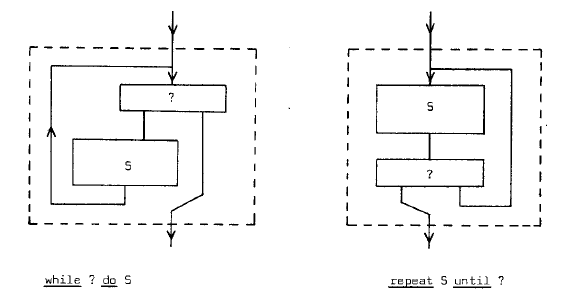
\includegraphics[width=.7\textwidth]{chap3/fig4}
	\caption{Tree form of syntax analyzer}
	\label{fig:syntax-analyzer-1}
\end{figure}

\begin{enumerate}[nosep, label=\arabic*.]
	\item \textbf{begin integer} $g$; $g\coloneq G[i, j, k]$;
	\item \label{en:comment-label-2}
	\quad \textbf{if} $g =$ ``$\perp$'' \textbf{then begin} good $\coloneq$ \textbf{true}; detach \textbf{end}
	
	\item \quad \textbf{else if} $g =$ symbol \textbf{then}
	
	\item \label{en:comment-label-4}
	\quad \textbf{begin} move right; match remainder; move left \textbf{end}
	
	\item \quad \textbf{else if} meta$(g)$ \textbf{then}
	
	\item \label{en:comment-label-6}
	\quad \textbf{begin} sub: $-$ \textbf{new} phrase$(g,$ sub$)$;
	\item \quad \quad \textbf{while} good \textbf{do}
	
	\item \label{en:comment-label-8}
	\quad \quad \textbf{begin} match remainder; call$($sub$)$ \textbf{end};
	
	\item \label{en:comment-label-9}
	\quad \quad sub: $-$ sub.left
	
	\item \quad \quad \textbf{end}
	\item \quad \textbf{end}
\end{enumerate}
\pagebreak[4]

\noindent
\textit{Comments}.

\begin{enumerate}[leftmargin=*, itemindent=2.2\parindent, nosep, label=Line \arabic*.]
	\item The $k$th symbol of the right hand side number $j$ is called $g$ for brevity.
	\item If $g$ is the terminator symbol the whole right-hand side has been successfully matched to the input. The object reports back to its master. Line \hyperref[en:comment-label-2]{2} does not alter the syntax tree or the position of the reading head.

	\setcounter{enumi}{3}
	\item Since we have a match the object moves the reading head to the next symbol. After having matched the remainder in all possible ways the
	object restores the position of the reading head. Thus, according to assumptions, line \hyperref[en:comment-label-4]{4} has a null net effect. 
	
	\setcounter{enumi}{5}
	\item Since $g$ is a meta-symbol, a new phrase object is generated to identify sub-phrases of the syntax class $g$. It becomes the new rightmost sub-phrase. Its left neighbor phrase is the old rightmost sub-phrase.
	
	\item We have assumed that an object when failing sets ``good'' to \textbf{false}.
	
	\item Since ``good'' is \textbf{true}, a sub-phrase has been identified matching $g$. After having matched the remainder in all possible ways, ``sub'' is 	called to identify the next possible sub-phrase. Since we want to match $g$ in all possible ways, line \hyperref[en:comment-label-8]{8} is repeated until the sub-phrase object fails.
	
	\item According to assumptions a phrase object which has failed, has had a null net effect. The total effect of lines \hyperref[en:comment-label-6]{6}\textendash\hyperref[en:comment-label-8]{8} is thus to add an object to the syntax tree. Line \ref{en:comment-label-9} restores the syntax tree to its original state.
\end{enumerate}

The comments show that the block above matches the symbol $g$ followed by the remainder of the $j$th right-hand side of $i$ in all possible ways and has a null net effect. Consequently the block itself satisfies the assumptions made for the ``match remainder'' statement. It follows that the whole matching algorithm may be expressed in a simple way by a recursive procedure. The whole computing process is described by the following class declaration.

\quad \textbf{class} phrase$(i$, left$)$; \textbf{integer} $i$; \textbf{ref} $($phrase$)$ left;

\quad \textbf{begin integer} $j$; \textbf{ref} $($phrase$)$ sub;

\quad \quad \textbf{procedure} match$(k)$; \textbf{integer} $k$;

\quad \quad \textbf{begin integer} $g$; $g\coloneq G[i,j, k]$;

\quad \quad \quad \textbf{if} $g =$ ``$\perp$'' \textbf{then begin} good $\coloneq$ \textbf{true}; detach \textbf{end}

\quad \quad \quad \textbf{else if} $g =$ symbol \textbf{then}

\quad \quad \quad \textbf{begin} move right; match$(k + 1)$; move left \textbf{end}

\quad \quad \quad \textbf{else if} meta$(g)$ \textbf{then}

\quad \quad \quad \textbf{begin} sub: $-$ \textbf{new} phrase $(g$, sub$)$;

\quad \quad \quad \quad \textbf{while} good \textbf{do}

\quad \quad \quad \quad \textbf{begin} match$(k + 1)$; call$($sub$)$ \textbf{end};

\quad \quad \quad \quad \quad sub: $-$ sub.left

\quad \quad \quad \quad \textbf{end}

\quad \quad \textbf{end} of match;

\quad \quad $j\coloneq 1$ \textbf{step} 1 \textbf{until} $jm[i]$ \textbf{do} match$(1);$

\quad \quad good $\coloneq$ \textbf{false}

\quad \textbf{end} of phrase

\noindent
A master program could have the following structure

\quad \textbf{ref} $($phrase$)$ tree;

\quad \dots

\quad tree: $-$ \textbf{new} phrase$($start, none$)$;

\quad \textbf{while} good \textbf{do begin} found: \dots; call$($tree$)$ \textbf{end};

\noindent
where ``start'' represents the start symbol of the grammar. At the label ``found'' a sentence has been identified and the variable ``tree'' refers to its syntax tree represented as described above. For each node its associated meta-symbol $(i)$, the rhs alternative number $(j)$, and the links to other nodes $($sub, left$)$ are available through remote identification, for example

\quad tree.$i$, tree.sub.$j$, tree.sub.left.left.sub.

We must expect in general that the strings matched by different successful trials may be of unequal lengths, starting at the same location of the tape. This may be avoided by defining the language in such a way that no initial segment of a valid text is also valid. Alternatively, the whole text should be followed by some symbol outside the alphabet, say ``$\perp$'', and the master program might have the following structure

\quad \textbf{ref} $($phrase$)$ parse; \textbf{Boolean} good;

\quad parse: $-$ \textbf{new} phrase $($start, \textbf{none}$)$;

\quad \textbf{while} good \textbf{do}

\quad \textbf{begin if} symbol $=$ ``$\perp$'' \textbf{then} inspect successful parse;

\quad \quad call$($parse$)$

\quad \textbf{end}

It is a remarkable feature of the phrase class that the result it yields on each call is a tree whose nodes consist in phrase objects which have been activated recursively and not yet terminated. Each of these phrase objects plays a dual role, both as a part of the syntactic tree which is to be inspected by the master program, and as the set of local variables for the recursive activation of other phrase objects. It is this close association of data and procedure which permits the algorithm to be so simply and concisely formulated.

Notice that each phrase object is the nucleus of a separate stack of recursive activation of its local ``match'' procedure. At the time when a detach is issued on behalf of an object, signaling a successful (sub-)parse, its stack has attained a temporary maximum depth, one level for each symbol in the current right-hand side, plus one level corresponding to the rhs terminator $\perp$, which issued the detach.

Thus the whole dynamic context of a successful parse is preserved. When an object is called to produce an alternative parse a backtracking process takes place, during which the ``match'' stack of the object is reduced. At a level corresponding to a meta-symbol in the rhs the match procedure calls on the corresponding phrase object to produce an alternative sub-parse (line \hyperref[en:comment-label-8]{8}) and so on. (cf. the row of officers in Chaplin's Great Dictator).

\section{Program concatenation}

In the preceding sections we have seen how the \textit{class} mechanism is capable of modeling certain simple concepts, by specifying data structures and defining operations over them. In this section, we develop a method by which more elaborate concepts can be constructed on the basis of simpler ones. This will establish potential hierarchies of concepts, with complex concepts subordinate to the more simple ones in terms of which they are defined. The structuring technique gives a new method of composing a program from its constituent parts, and is known as \textit{concatenation}.

Concatenation is an operation defined between two classes $A$ and $B$, or a class $A$ and a block $C$, and results in formation of a new class or block. Concatenation consists in a merging of the attributes of both components, and the composition of their actions. The formal parameters of the concatenated object consist of the formal parameters of the first component followed by formal parameters of the second component; and the same for specification parts, declarations and statements (if any).

A concatenated class $B$ is defined by prefixing the name of a first component $A$ to the declaration of $B$:

\quad $A$ \textbf{class} $B(b_1, b_2, \dots)$; \dots specification of $b$'s;

\quad\quad \textbf{begin}\dots attributes of $B$\dots; \dots actions of $B$\dots \textbf{end}

\noindent
Suppose the class $A$ has been defined:

\quad \textbf{class} $A(a_1, a_2 , \dots)$; \dots specification of $a$'s\dots;

\quad \quad \textbf{begin}\quad attributes of $A$\dots; \dots actions of $A$\dots \textbf{end}.

According to the concatenation rules, the effect of the prefixed declaration
for class $B$ is the same as if $B$ had been declared without a prefix thus:

\quad \textbf{class} $B(a_1, a_2, \dots, b_1, b_2, \dots)$; \dots specification of $a$'s\dots

\quad \quad \quad specifications of $b$'s\dots;

\quad \quad \textbf{begin}\dots attributes of $A$\dots; \dots attributes of $B$\dots;

\tabto*{5.9em}\dots statements of $A$\dots; \dots statements of $B$\dots \textbf{end};

\textit{Note}. If any local identifiers of $A$ are the same as local identifiers of $B$, the collision of names is resolved by systematic change of $B$'s identifiers. A block also may be prefixed by a class identifier:

\quad $A$ \textbf{begin} declarations\dots; \dots statements \textbf{end},

\noindent
and the effect is similar to that described above, except that the result of the concatenation is a block, not a class. (If the class $A$ has parameters, the prefix must include an actual parameter part 1). The effect of prefixing a block is to make available within that block the library of procedures and related data (including even classes) declared within the class declaration for $A$.

A single class may be used as prefix to several different concatenated classes. For example, suppose a program requires to deal with trucks, buses, and private cars. These are three separate classes, and each has its own attributes. But there are certain attributes (for example license number) which are common to all of them, by virtue of the fact that they are all vehicles. The concept of vehicle is a more general one, and could be declared as a separate concept;

\quad \textbf{class} vehicle$($license no$)$; \textbf{integer} license no; \dots;

\noindent
This class can now be used as a prefix in the remaining class declarations.

\quad vehicle \textbf{class} truck (load); \textbf{real} load; \dots;

\quad vehicle \textbf{class} bus (seating); \textbf{integer} seating; \dots;

\quad vehicle \textbf{class} car; \dots;

An object belonging to a prefixed class is a compound object, which has certain attributes and operations \textit{in addition to} those defined in the prefix part. Thus a truck object has a license no and a load, and a bus object has a license no and a seating. It is reasonable to regard ``truck'' and ``bus'' and ``car'' as \textit{subclasses} of the vehicle class; any object of a subclass also belongs to the prefix class ``vehicle''.

A reference variable may be qualified as belonging to a prefix class or to a concatenated class. If it belongs to the prefix class it may point to objects of \textit{any} of the subclasses, and may be used in a remote identifier to access any of the attributes of the prefix class but not to access any attributes of the subclasses. A reference qualified by a subclass may point only to objects of the subclass, but may be used in a remote identifier to access all its attributes. Thus given the reference variables:

\quad \quad \textbf{ref} $($vehicle$)\ V$; \textbf{ref} $($bus$)\ B$;

\quad the following are valid remote identifiers:

\quad \quad $V$.license no, $B$.license no, $B$.seating,

\quad but $V$.seating is not valid.

\noindent
Thus the subclass notion provides a useful flexibility of object referencing. A ``weak'' qualification permits a wide range of objects referencing, at the cost of inability to make remote access to attributes declared in a subclass.

Assignment of a subclass reference to a prefix class reference variable $($e.g. $V$: $-\ B)$ is always valid, and can be recognized as such at compile time. But assignment in the other direction $($e.g. $B$: $-\ V)$ may give rise to an error (detected only at run time), if the object referenced does not in fact belong to the expected subclass (bus).

\subsection{Binary search tree}

Suppose it is desired to set up a binary search tree to hold information about stock items in an inventory. Each node of the tree should contain not only a val (indicating the stock number of the item) but also certain other information. about quantity on hand, price, reorder point, etc. The simplest way of achieving the required effect is to prefix the class ``stock item'' by the class tree, and then declare the additional attributes required, for example:

\quad tree \textbf{class} stock item;

\quad \quad \textbf{begin integer} $qoh$, price, reorder point;

\quad \quad \quad \textbf{Boolean} ordered;

\quad \quad \quad \textbf{procedure} reduce;

\quad \quad \quad \quad \textbf{begin if} $qoh =$ reorder point \& $\neg$, ordered \textbf{then}

\quad \quad \quad \quad \quad issue reorder;

\quad \quad \quad \quad \quad $qoh \coloneq qoh -1$

\quad \quad \quad \quad \textbf{end} of remove;

\quad \quad \textbf{end} of stock item;

\subsection{Two way list}

Taking advantage of the concatenation technique, it is possible to design classes which are intended solely or primarily to act as prefixes to other classes or to blocks. In this section we give an example of a class TWLIST, which is intended to be used as a prefix to a block, and to make available within that block the concept of two-way chained cyclic lists. Such a list consists of a \textit{list head}, which contains two pointers, one to the first element of the chain and one to the last. Each \textit{link} in the chain must also contain two pointers, suc which points to the successor in the list (or the list head if there is none), and pred which points to the predecessor in the list (or the list head if there is none). In an empty list, the two pointers from the list head point to the list head itself.

Each pointer in the system must be capable of pointing either to another link in the list or to a list head. Therefore these pointers must be qualified by a class which embraces both links and heads, i.e. a class ``linkage'' of which they are both subclasses. Since both list heads and links require two reference attributes, suc and pred can be declared as attributes of the prefix class linkage.

The single concept of a two-way list is represented by the triple of classes linkage, link, and list head. In order to indicate that they are to be considered in conjunction as a single concept, the declarations for all three classes are grouped together in a single class declaration TWLIST, which is to be used as a prefix to any block which requires to use the concept. Within such a block the ``link'' class is intended to be used as a prefix to other classes specifying the nature of the items; for example, if stock items were to be held in a two-way list instead of in a binary search tree, the declaration would be:

\quad link \textbf{class} stock; \dots as before\dots;

It is now necessary to decide on a basic set of operations on lists and links. A link $I$ should be removable from its list by a procedure statement

\quad $I$.out;

\noindent
and it should be capable of being reinserted in a list just before link $J$ by a procedure statement:

\quad $I$.precede$(J)$;

\noindent
Since a link can belong to at most one list, this operation should also remove $I$ from any list it happens to belong to before. Finally a link should be insertable as the last item of a list with head $H$ by a procedure statement:

\quad $I$.into$(H)$;

For a list head $H$, it seems useful to define the following functions

\quad $H$.empty,

\noindent
which tests whether the list is empty,

\quad $H$.first

\noindent
which yields $H$'s first item, if any; otherwise \textbf{none}, and

\quad $H$.last

\noindent
which yields $H$'s last item, if any; otherwise \textbf{none}.

The declaration of the class TWLIST can now be given:

\begin{enumerate}[nosep, label=\arabic*.]
	\item \textbf{class} TWLIST;
	\item \textbf{begin class} linkage; \textbf{begin ref} $($linkage$)$ suc, pred; \textbf{end};
	\item \quad linkage \textbf{class} link;
	\item \quad \textbf{begin procedure} out;
	\item \quad \quad \textbf{if} suc $=/=$ \textbf{none then}
	\item \quad \quad \textbf{begin} suc.pred: $-$ pred; pred.suc: $-$ suc;
	\item \quad \quad \quad suc: $-$ pred: $-$ \textbf{none}
	\item \quad \quad \textbf{end} of out;
	\item \quad \quad \textbf{procedure} precede$(x)$; \textbf{ref} $($linkage$)\ x$;
	\item \quad \quad \textbf{begin} out; suc: $-\ x$; pred: $-\ x$.pred;
	\item \quad \quad \quad suc.pred: $-$ pred.suc: $-$ \textbf{this} link
	\item \quad \quad \textbf{end} of precede;
	\item \quad \quad \textbf{procedure} into $(L)$; \textbf{ref} $($list$)\ L$;
	\item \quad \quad \quad precede$(L)$;
\end{enumerate}

\hangindent=2.9\parindent\quad \quad \quad \textbf{comment} suc and pred of a link object should have the standard initial value \textbf{none} indicating no list membership;

\begin{enumerate}[nosep, label=\arabic*.]
	\setcounter{enumi}{14}
	\item \quad \textbf{end} of link;
	\item \quad linkage \textbf{class} list;
	\item \quad \textbf{begin ref} $($link$)$ \textbf{procedure} first;
	\item \quad \quad \quad first: $-$ \textbf{if} empty \textbf{then none else} suc;
	\item \quad \quad \textbf{ref} $($link$)$ \textbf{procedure} last;
	\item \quad \quad \quad last: $-$ \textbf{if} empty \textbf{then none else} pred;
	\item \quad \quad \textbf{Boolean procedure} empty;
	\item \quad \quad \quad empty: $=$ suc $==$ \textbf{this} list;
	\item \quad \quad \quad suc: $-$ pred: $-$ \textbf{this} list
\end{enumerate}

\hangindent=3.6\parindent\quad \quad \quad \quad \textbf{comment} suc and pred of a list head should be initialized to indicate an empty list;

\begin{enumerate}[nosep, label=\arabic*.]
	\setcounter{enumi}{14}

	\item \quad \textbf{end} of list;
	\item \textbf{end} of TWLIST;
\end{enumerate}

Let $P$ be an \textit{arbitrary} block instance prefixed by TWLIST, which, outside its prefix part, contains no explicit reference assignment to any variable suc or pred of any linkage object. Then the assertions \ref{en:twlist-1} and \ref{en:twlist-2} below are valid throughout the lifetime of $P$ (at times when control is textually outside the body of TWLIST).

\begin{enumerate}[wide, nosep, label=(\arabic*)]
	\item \label{en:twlist-1}
	Any linkage object $x$ in $P$ is either an object with no list membership, in which case $x$.suc $== x$.pred $==$ \textbf{none} and $x \notin$ list, or $x\text{.suc.pred} == x\text{.pred.suc} == x$. 
	
	It follows that all lists contained in $P$ are circular. Furthermore:
	
	\item \label{en:twlist-2}
	Each circular list in $P$ contains exactly one list head, which is an object of the class ``list''.
\end{enumerate}

The assertions are established by observing that each of the operations
below preserves their validity, and that P contains no linkage object initially.

\noindent
\textbf{new} \textit{link} (or \textbf{new} $C$, $C \subseteq$ linkage-list) generates a link object, which is not a list member (its suc and pred are automatically initialized to \textbf{none}).

\noindent
\textbf{new} \textit{list} (or \textbf{new} $C$, $C \subseteq$ list) generates an ``empty'' circular list containing the generated list head and initially nothing else.

\noindent
In the following we assume $x \in \text{link}$, $y$, $z \in \text{linkage}$, and $L \in \text{list}$. $x \leftrightarrow y$ is an abbreviation for $x.\text{suc} == y$ \& $x == y$.pred.

\noindent
$x.out$ If $z \leftrightarrow x \leftrightarrow y$ the result is $z \leftrightarrow y$ and $x$ is not a list member. (Notice that \ref{en:twlist-2} together with $x$ e link implies $x =/= y$, $z$.) If $x$ was not a list member, the result is to do nothing.

\noindent
$x.precede(y)$, where $x =/= y \land z \leftrightarrow y$. The result is $x \leftrightarrow y$ (and $z \leftrightarrow x$ if $x =/= z$). If $x$ was a list member, $x$ is first removed from that list.

\noindent
$x.into(L)$, where $z \leftrightarrow L$. The result is $z \leftrightarrow x \leftrightarrow L$, which implies $x == L$. last. If $x$ was a list member, $x$ is first removed from that list.

Any use of out, precede, or into not satisfying the above assumptions, is either textually illegal or leads immediately to a run time error and program termination caused by an invalid remote identifier. E.g. the operation $x$.precede$(y)$ sets $x$.pred to \textbf{none} if $x == y$ or $y$ is not a list member. Consequently the remote identifier pred. suc in the body of precede is invalid. Notice that $x$.into$(L)$ is a ``safer'' operation, since $x$ e link, $L \in \text{list}$ implies that $x =/= L$ and $L.\text{pred} =/= \text{\textbf{none}}$.

The assertions \ref{en:twlist-1} and \ref{en:twlist-2} provide a guarantee that our lists are well behaved, provided that no explicit assignment to any variable suc or pred occurs. The construction TWLIST is thus a reliable ``mental platform,'' which in a certain sense \textit{cannot break down}, whatever programming errors are made. When programming on top of TWLIST one is entitled to ignore the list processing details involved in manipulating the circular two-way lists. Each list object may be regarded as representing an \textit{ordered set} of link objects, with the proviso that a link object may be member of at most one such set at a time. The last fact is reflected in the design of the procedures into and.precede. Explicit use of the attributes suc and pred, e.g. for scanning through a list, may, however, require the user to be conscious of the fact that the ``last'' member has a successor and the ``first'' member a predecessor, which are both identical to the list object itself. A design alternative is to suppress this fact by declaring the following procedures as attributes to link.

\quad \textbf{ref} $($link$)$ \textbf{procedure} successor;

\quad \quad \textbf{inspect} suc \textbf{when} list \textbf{do} successor: $-$ \textbf{none}

\quad \quad \textbf{otherwise} successor: $-$ suc;

\quad \textbf{ref} $($link$)$ \textbf{procedure} predecessor;

\quad \quad \textbf{inspect} pred \textbf{when} list \textbf{do} predecessor: $-$ \textbf{none}

\quad \quad \textbf{otherwise} predecessor: $-$ pred;

Note the construction

\quad \textbf{inspect} $r$ \textbf{when} $C$ \textbf{do}\dots

\noindent
enables the programmer to test whether the object referenced by r belongs to one of its possible subclasses $C$.

\section{Concept Hierarchies}

At the outset of a programming project there is a \textit{problem}, more or less precisely defined and understood in terms of certain problem oriented concepts, and a \textit{programming language}, perhaps a general purpose one, providing some (machine oriented) basic concepts, hopefully precisely defined and completely understood. There is a \textit{conceptual distance} between the two, which must be bridged by our piece of program. We may picture that distance as a vertical one, the given programming language being the ground level.

Our difficulty in bridging such gaps is the fact that we have to work sequentially on one simple part problem at a time, not always knowing in advance whether they are the \textit{right problems}.

In order to better overcome such difficulties we may build pyramids. Unlike the Egyptian ones ours are either standing on their heads (bottom-up construction) or hanging in the air (top-down construction). The construction principle involved is best called \textit{abstraction}; we concentrate on features common to many phenomena, and we abstract \textit{away} features too far removed from the conceptual level at which we are working. Thereby we have a better chance of formulating concepts which are indeed useful at a later stage.

In the bottom-up case we start at the basic language level and construct abstract concepts capable of capturing a variety of phenomena in some problem area. In the top-down case [\hyperref[ref:8]{8}, \hyperref[ref:9]{9}] we formulate the solution to a given problem in terms of concepts, which are capable of being implemented (and interpreted) in many ways, and which are perhaps not yet fully understood. In either case system construction may consist of adding new layers of pyramids (above or below) until the conceptual gap has finally been bridged. Each such layer will correspond to a conceptual level of understanding.

For instance, given some problem which involves queueing phenomena, we could take TWLIST of the preceding section as the first step of a bottom-up construction. Then, for the remainder of the construction we are free to think and express ourselves in terms of dynamic manipulation of ordered sets of 
objects.

Layers of conceptual levels may be represented as a \textit{prefix sequence} of class declarations. For example, it is possible to construct a series of class declarations, each one using the previous class as prefix

\hfill\textbf{class} $C_1$; \dots;\hspace{14em}

\hfill $C_1$ \textbf{class} $C_2;$ \dots;\hspace{14em}

\tabto*{13em}\dots

\hfill $C_{n - 1}$ \textbf{class} $C_n$; \dots;\hspace{14em}

\noindent
The list $C_1, C_2, \dots, C_{n-1}$ is known as the prefix sequence for $C_n$. The outermost prefix $C_1$ is built at the ground level. Every other level rests on the one(s) below, in that it may take advantage of all attributes of its entire prefix sequence. Making use of this language mechanism, bottom-up construction of a program is to plan and write the classes of a prefix sequence one by one in the stated order. The program itself is finally written as a prefixed block on top of the whole sequence.

\quad $C_n$ \textbf{begin} \textemdash{} \textbf{end}

\noindent
The top-down strategy would correspond to constructing the members of the prefix sequence, including the prefixed block, in the reverse order. (SIMULA 67 contains additional mechanisms, not considered here, for facilitating top-down and mixed mode construction.)

A well-formed conceptual level (bottom-up) is a set of well-defined interrelated concepts, which may be combined to make more elaborate concepts. It may serve for further construction as a mental platform, raised above ground towards some application area, i.e. as an ``application language''. A preconstructed application language may serve to shorten the conceptual gap that has to be bridged for many problems in the area. The usefulness of such a platform is closely related to its ruggedness, that is with the way in which it tolerates or even forestalls misuse. As we saw in the last section TWLIST supplies an exceptionally rugged mental platform; and in this section we shall build on it a small but useful application language, which may in its turn be used as a platform for the solution of realistic problems.

\subsection{Discrete event simulation}

Simulation is a method for studying the behavior of large systems of interacting objects, and evaluating the effect of making changes which would be too expensive to make on an experimental basis in real life. The object of a simulation model could be a production line, a traffic system, a computer system (hardware and software), a social system composed of interacting individuals, etc. The following notions are common to most such systems.

\begin{enumerate}[wide, nosep, label=(\arabic*)]
	\item Processes taking place in \textit{parallel}, giving rise to discrete events at irregular intervals of time.
	\item \textit{Queueing} phenomena, arising when an object has to wait for service from a currently busy server.
\end{enumerate}

In order to represent processes occurring in parallel, it is not necessary that the corresponding program components should be multiprogrammed in the computer; but it is necessary that the programs should be able to suspend themselves temporarily, and be resumed later from where they left off. Thus the active objects or ``processes'' in a simulation will be represented by (semi-)coroutines, operating in \textit{pseudo-parallel} under control of a scheduling mechanism.

For example, in a job shop simulation, an incoming order gives rise to a sequence of events on the shop floor, to satisfy the order. Each order may be regarded as a process whose activity is to proceed from one machine to the next, requesting and obtaining service from it. The sequence of requests is determined by the nature of the order. If the requested machine is free, the order is served immediately, and the machine goes busy for a period equal to the length of the service. Otherwise, the order joins a queue of orders waiting for the machine to become free.

In the implementation of the concept of simulated time, the first requirement is that each process have access to a variable ``time'' which holds the current time, and which is incremented on appropriate occasions by the time-control mechanism. Note that the updating of this variable must be entirely independent of the passage of computing time during the simulation, since actions which take a long time on a computer might take only a short time in the real world, and vice versa. As far as simulated time is concerned, the active phases of the processes must be instantaneous; ``time'' does not move until all the participating processes are passive.

Thus in order to simulate the passing of time, a process simulating an active system component must relinquish control for a stated interval $T$ of simulated time; and it must be reactivated again when the time variable has been incremented by $T$. This will be accomplished by the process calling the procedure

\quad hold$(T)$.

For example, an order which has found its required machine ready to serve it needs to indicate how long this service will take, by the statement

\quad hold$($service interval$)$;

\noindent
The order will now become inactive until all other orders which were due to be reactivated \textit{before} time $+$ service interval have been reactivated, and have relinquished control again. At this point, the given order will be reactivated, and will find that its time has been appropriately incremented.

While a process is held, it will be necessary to record its reactivation time as one of its attributes. It is convenient therefore to use the time attribute of the process itself for this purpose.

The method of holding for a specified interval is possible only if the process knows how long it has to wait before the next ``event'' in its life. But sometimes it may require to wait until the occurrence of some event in the life of some other process. For example, an order, on finding its required machine busy, must join a queue and wait until the machine is free; and an order on releasing a machine must activate the first other order in the queue (if not empty). Thus two additional procedures are required:

\quad wait$(Q)$,

\quad and activate$(X)$,

\noindent
where $Q$ refers to the queue (two-way list) on which the calling process is to wait while it is passive, and $X$ refers to some passive process. which is to be removed from its queue and allowed to proceed.

Finally, a means must be provided of starting and stopping the simulation. This may be accomplished by a procedure statement

\quad simulate$($start, finish$)$,

\noindent
where start refers to the process with which the simulation starts, and finish gives the time limit for the simulation. Any process requesting to be held beyond this limit may be ignored. Presumably, the start process will activate other processes to participate in the simulation.

We now proceed to implement the mechanism described above. It will be implemented as a class MINISIM, which is intended to be used as a prefix to a simulation main program. In order to take advantage of the two-way list mechanism, the MINISIM class must be prefixed by TWLIST. This ensures that TWLIST is also available in any simulation program which is prefixed by MINISIM.

A class of objects which are to be capable of participating in a simulation should be declared as a subclass of the ``process'' class. This will make available to it the necessary time control and queueing mechanisms. Each process must have the capability of inserting itself into a two-way list; therefore the process class itself must be declared as a subclass of the class of links.

Processes waiting for the elapse of their holding interval are held on a unique two-way list known as the sequencing set (\textit{SQS}). The processes are ordered in accordance with decreasing reactivation times. A specially created finish process is always the first link in \textit{SQS}, and the last link is always the one that is currently active. Its time represents the current time of the system. When it goes inactive, its predecessor in the \textit{SQS} will (usually) become the last, and its local time has already been updated to the time at which that process was due to be reactivated.

We are now in a position to give the general structure of MINISIM, omitting for the time being the procedure bodies.

\quad TWLIST \textbf{class} MINISIM

\quad \textbf{begin ref} $($list$)$ \textit{SQS};

\quad \quad \textbf{ref} $($process$)$ \textbf{procedure} current;

\quad \quad \quad current: $-$ \textit{SQS}.last;

\quad \quad \quad link \textbf{class} process;

\quad \quad \quad \quad \textbf{begin real} time;

\quad \quad \quad \quad \quad \textbf{procedure} hold$(T)$; \textbf{real} $T$;

\quad \quad \quad \quad \quad \quad \dots;

\quad \quad \quad \quad \quad \textbf{procedure} wait$(Q)$; \textbf{ref} $($list$)\ Q$;

\quad \quad \quad \quad \quad \quad \dots;

\quad \quad \quad \quad \quad \textbf{procedure} activate$(X)$; \textbf{ref} $($process$)\ X$;

\quad \quad \quad \quad \quad \quad \dots;

\hangindent=4.25\parindent\quad \quad \quad \quad \quad detach; \textbf{comment} a new process doesn't actually do anything until it is activated

\quad \quad \quad \quad \textbf{end} of process;

\quad \quad \quad \textbf{procedure} simulate$($start, finish$)$;

\quad \quad \quad \quad \textbf{ref} $($process$)$ start; \textbf{real} finish;

\quad \quad \quad \quad \quad \dots;

\quad \quad \textbf{end} of MINISIM.

\noindent
We shall give the bodies of the procedures in reverse order.

\quad simulate: \textbf{begin} \textit{SQS}: $-$ \textbf{new} list;

\quad \quad \textbf{new} process.into $(SQS)$; current.time $\coloneq$ finish;

\quad \quad \quad \textbf{if} start.time $<$ finish \textbf{then} start.into$(SQS)$;

\quad \quad \quad \textbf{while} $\neg SQS$.empty \textbf{do}

\quad \quad \quad \quad \textbf{begin} call$($current$)$;

\quad \quad \quad \quad \quad current.out;

\hangindent=4.25\parindent\quad \quad \quad \quad \quad \textbf{comment} this ensures that a terminated or detached process leaves the $SQS$;

\quad \quad \quad \quad \textbf{end}

\quad \quad \textbf{end} of simulate

\quad wait: \textbf{begin} into$(Q)$; resume$($current$)$ \textbf{end};

\noindent
The active process inserts itself into the queue, and thereby leaves the $SQS$. It also resumes the process on the $SQS$ which is next due to be reactivated. Notice that the standard sequencing mechanism of the simulate procedure must be bypassed, since the old active process already is out of the $SQS$.

\quad activate: \textbf{begin} $X$.into$(SQS)$; \textbf{comment} as its last and current member;

\quad \quad $X$.time $\coloneq$ time; \textbf{comment} i.e. now;

\quad \quad resume$($current$)$;

\quad \textbf{end} of activate.

\noindent
The calling process places $X$ ahead of itself in $SQS$, but with the same time. Since the calling and the activated process $X$ have the same time, it does not matter to the timing mechanism in what order they are placed; our choice implies that an active phase of $X$ is invoked immediately in real time. Control returns to the calling one at the same moment of simulated time, but after the completion of the active phase of $X$.

\quad hold:

\quad \textbf{begin ref} $($process$)\ P$;

\quad \quad $P$: $-$ pred;

\hangindent=3\parindent\quad \quad \textbf{comment} the holding process is necessarily active, and therefore also the last member of $SQS$. Since the finish process never holds, there will always be a second-to-last process on $SQS$

\quad \quad \textbf{if} $T > 0$ \textbf{then} time $\coloneq \text{time} + T$;

\quad \quad \textbf{comment} set local reactivation time, time should never decrease;

\quad \quad \textbf{if} time $\geqslant P$.time \textbf{then}

\quad \quad \quad \textbf{begin comment} this process must be moved in $SQS$;

\quad \quad \quad \quad out; \textbf{comment} of $SQS$, now $P$ is current;

\quad \quad \quad \quad $P$: $-\ SQS$.first; \textbf{comment} the finish process;

\quad \quad \quad \quad \textbf{if} time $< P$.time \textbf{then}

\quad \quad \quad \quad \quad \textbf{begin comment} reactivation time is within the time limit;

\quad \quad \quad \quad \quad \quad \textbf{while} time $< P$.time \textbf{do} $P$: $-\ P$.suc;

\quad \quad \quad \quad \quad \quad \textbf{comment} terminates since time $\geqslant$ current.time;

\quad \quad \quad \quad \quad \quad precede$(P)$

\quad \quad \quad \quad \quad \textbf{end}; \textbf{comment} ignore a process that would exceed the limit;

\quad \quad \quad \quad resume$($current$)$

\quad \quad \textbf{end};

\quad \textbf{end} of hold;

\noindent
Notice that a process object is allowed to relinquish control simply by saying detach or by passage through its \textbf{end}. In both cases control returns to the standard sequencing mechanism of the simulate procedure. The basic activation instructions call and resume, however, should not be explicitly applied to process objects; that would illegally bypass the timing mechanism.

\subsection{The Lee Algorithm}

As a simple but unexpected example of the use of simulated time, we take the Lee algorithm for finding the shortest path between a city $A$ and a city $B$ connected by a network of one-way roads. The algorithm may be envisaged as the propagation of a pulse from the destination city $B$ at equal speed along all roads leading into it. Each time a pulse reaches a city not reached by a previous pulse, it records the road it has come along, and then sends pulses outward along all roads leading into the city. When a pulse reaches a city which has already been reached by another pulse, it dies. When a pulse reaches the city $A$, the task is completed.

Cities and roads may be represented by classes.

\quad \textbf{class} city; \textbf{begin ref}$($road$)$ roadsin, wayout; \dots \textbf{end}

\quad \textbf{class} road; \textbf{begin real} length; \textbf{ref} $($road$)$ nextin;

\quad \quad \textbf{ref} $($city$)$ source, destination; \dots \textbf{end}

\noindent
The variable wayout holds the recommended wayout from the city towards $B$. For an unvisited city, its value is \textbf{none}.

The class representing a pulse takes as parameter the road along which it is first to pass.

\quad \textbf{process class} pulse$(rd)$; \textbf{ref} $($road$)\ rd$;

\quad \textbf{begin ref} $($city$)\ c$; $c$: $-\ rd$.source;

\quad \quad hold$(rd$.length$)$;

\quad \quad \textbf{if} $c$.wayout $=/=$ \textbf{none then}

\quad \quad \textbf{begin} $c$.wayout: $-\ rd$;

\quad \quad \quad \textbf{if} $c == A$ \textbf{then go to} done;

\quad \quad \quad \textbf{comment} stops the simulation by going to a non-local label;

\quad \quad \quad $rd$: $-\ c$.roadsin;

\quad \quad \quad \textbf{while} $rd$ $=/=$ none \textbf{do}

\quad \quad \quad \textbf{begin} activate$($\textbf{new} pulse $(rd));$

\quad \quad \quad \quad $rd$: $-$ $rd$.nextin

\quad \quad \quad \textbf{end} propagation of pulses

\quad \quad \textbf{end}

\quad \textbf{end} of pulse

The algorithm will be invoked by calling a procedure with parameters indicating the starting and final cities, and an upper limit $L$ on the length of the path that is to be printed. It is assumed that the wayout of every city is initially \textbf{none}. The time and process concepts are made available by the prefix MINISIM to the procedure body.

\quad \textbf{procedure} Lee$(A, B, L)$; \textbf{ref} $($city$)\ A, B$; \textbf{real} $L$;

\quad \quad MINISIM \textbf{begin} process \textbf{class} pulse$(rd)$; \textbf{ref} $($road$)\ rd$;

\quad \quad \quad \dots as \textbf{before}\dots;

\quad \quad \quad process \textbf{class} starter;

\quad \quad \quad \quad \textbf{begin ref} $($road$)\ rd$;

\quad \quad \quad \quad \quad $rd$: $-\ B$.roadsin;

\quad \quad \quad \quad \quad \textbf{while} $rd =/=$ \textbf{none do}

\quad \quad \quad \quad \quad \quad \textbf{begin} activate $($\textbf{new} pulse$(rd))$;

\quad \quad \quad \quad \quad \quad \quad \quad $rd \coloneq rd$.nextin

\quad \quad \quad \quad \quad \quad \textbf{end}

\quad \quad \quad \quad \textbf{end} of starter;

\quad \quad \quad \quad simulate$($\textbf{new} starter, $L)$;

\quad \quad done: \textbf{end} of Lee;

\noindent
After a procedure statement such as

\quad Lee $($Oslo, Belfast, 1000$)$;

\noindent
where \textbf{ref} $($city$)$ Oslo, Belfast; the required route may be printed out, provided that it exists.

\quad \textbf{if} Oslo.wayout $=/=$ \textbf{none then}

\quad \textbf{begin ref} $($city$)\ c$; \textbf{procedure} print\dots; \dots;

\quad \quad print$($Oslo.wayout$)$; $c$: $-$ Oslo.wayout.destination;

\quad \quad \textbf{while} $c =/=$ Belfast \textbf{do}

\quad \quad \textbf{begin} print$(c)$; print$(c$.wayout$)$;

\quad \quad \quad $c$: $-\ c$.wayout.destination

\quad \quad \textbf{end}

\quad \textbf{end else} outtext$($'no road connection within limit$)$;

\noindent
It is assumed for the print procedure that cities and roads are objects belonging to a common class, by having the same prefix to the two classes. The prefix part of an object might contain the necessary identifying text, such as `London' or `M1' as data.

\subsection{A job shop model}

As a second application of MINISIM we shall design a model of a simple job shop system. The model may be used to evaluate the capacity of the shop in relation to a given order load. The line numbers below refer to the program on page \pageref{pg:program-job-shop}.

The system consists of \textit{machine groups} (lines \hyperref[pg:program-job-shop-3]{3}\textendash \hyperref[pg:program-job-shop-10]{10}), numbered from 1 to \textit{nmg} (lines \hyperref[pg:program-job-shop-1]{1}, \hyperref[pg:program-job-shop-11]{11}), and \textit{order} objects (lines \hyperref[pg:program-job-shop-12]{12}\textendash \hyperref[pg:program-job-shop-22]{22}). The machines of a group are identical and therefore need not be represented individually; however, theirnumber is specified initially by the value of the attribute \textit{nm} (line \hyperref[pg:program-job-shop-3]{3}). Associated with the group is also a queue of orders waiting to be processed, which is empty initially (lines \hyperref[pg:program-job-shop-4]{4}, \hyperref[pg:program-job-shop-9]{9}), and procedures to \textit{request} a machine for processing (lines \hyperref[pg:program-job-shop-5]{5}\textendash \hyperref[pg:program-job-shop-6]{6}) and to \textit{release} it when finished (lines \hyperref[pg:program-job-shop-7]{7}\textendash \hyperref[pg:program-job-shop-8]{8}).

The variable \textit{nm} is used to represent the number of available machines, say $m$, as well as the number of orders, say $w$, waiting in the queue, as described by the following assertion.

\quad \textbf{if} $nm > 0$ \textbf{then} $m = nm \land w = 0$

\quad \textbf{else} $m = 0 \land w = \text{abs}(nm)$

\noindent
The assertion is valid for each machine group (outside the procedure bodies request and release).

When a machine is requested and $m = 0$, the caller must enter the queue and wait for its turn (line \hyperref[pg:program-job-shop-6]{6}). When a machine is released and $w \neq 0$, one of the waiting processes should proceed. The first member of the queue is activated and thereby leaves the queue. The queueing discipline is thus first come first served.

The orders are process objects, each of which generates its successor, (line \hyperref[pg:program-job-shop-18]{18}) and which goes from one machine group to the next (lines \hyperref[pg:program-job-shop-20]{20}\textendash \hyperref[pg:program-job-shop-21]{21}) according to an individually defined schedule. For a given order the schedule has $n$ steps, and for each step $s(s = 1, 2, \dots, n)$ a machine group number $(mg[s])$ and an associated processing time $(pt[s])$ are given. Thus the order should spend the time $pt[s]$ in being processed at machine group number $mg[s]$ (line \hyperref[pg:program-job-shop-21]{21}, hold). Notice that the request statement of line \hyperref[pg:program-job-shop-21]{21} will require some additional amount of simulated time for its completion, if the group $m$group$[mg[s]]$ currently has no available machine.

The model is driven by input data. In particular, each order object during its first active phase reads in its own schedule, consisting of length of schedule (line \hyperref[pg:program-job-shop-18]{18}) arrival time (inreal, line \hyperref[pg:program-job-shop-15]{15}), and the values of $mg$ and $pt$ (lines \hyperref[pg:program-job-shop-16]{16}\textendash\hyperref[pg:program-job-shop-17]{17}). The main program sets up machine groups of specified sizes (lines \hyperref[pg:program-job-shop-24]{24}, \hyperref[pg:program-job-shop-25]{25}) and generates the first order at time zero. (The procedures inint, inreal, and lastitem are procedures associated with a standard input file, which is part of the program environment).

It is assumed that the input file starts with the following data:

\quad $nmg, \text{timelimit}, nm_1, nm_2, \dots, nm_{nmg}$

\noindent
defining the structure of the job shop; and this is followed by an occurrence of

\quad $n, T, mg_1, pt_1, mg_2, pt_2, \dots, mg_n, pt_n,$

\noindent
for each order to be generated. Each value $T$ defines the arrival time of the order. It is assumed that the $T$ values are in a non-decreasing sequence.

The JOB SHOP goes as follows.

\begin{enumerate}[nosep, label=\arabic*.]
	\label{pg:program-job-shop}
	
	\item \label{pg:program-job-shop-1}
	\textbf{begin integer} $nmg;\ nmg \coloneq$ inint;
	 
	\item MINISIM \textbf{begin}
	
	\item \label{pg:program-job-shop-3}
	\textbf{class} machine group$(nm)$; \textbf{integer} $nm$;
	
	\item \label{pg:program-job-shop-4}
	\textbf{begin ref} $($list$)\ Q$;
	
	\item \label{pg:program-job-shop-5}
	\quad \textbf{procedure} request;
	
	\item \label{pg:program-job-shop-6}
	\quad \textbf{begin} $nm \coloneq nm - 1$; \textbf{if} $nm < 0$ \textbf{then} current.wait$(Q)$ \textbf{end};
	
	\item \label{pg:program-job-shop-7}
	\quad \textbf{procedure} release;
	
	\item \label{pg:program-job-shop-8}
	\quad \textbf{begin} $nm \coloneq nm + 1$; \textbf{if} $nm \leqslant 0$ \textbf{then} current.activate$(Q$.first$)$ \textbf{end};
	
	\item \label{pg:program-job-shop-9}
	\quad $Q$: $-$ \textbf{new} list
	
	\item \label{pg:program-job-shop-10}
	\textbf{end} of machine group;
	
	\item \label{pg:program-job-shop-11}
	\textbf{ref} $($machine group$)$ \textbf{array} $m$group$[1:nmg]$;
	
	\item \label{pg:program-job-shop-12}
	process \textbf{class} order$(n)$; \textbf{integer} $n$;
	
	\item \label{pg:program-job-shop-13}
	\textbf{begin integer array} $mg[1:n]$; \textbf{array} $pt[1:n]$; \textbf{integer} $s$;
	
	\item \label{pg:program-job-shop-14}
	\quad \textbf{ref} $($machine group$)\ M$;
	
	\item \label{pg:program-job-shop-15}
	\quad hold$($inreal $-$ time$)$; \textbf{comment} arrival time is now;
	
	\item \label{pg:program-job-shop-16}
	\quad \textbf{for} $s\coloneq 1$ \textbf{step} 1 \textbf{until} $n$ \textbf{do}
	
	\item \label{pg:program-job-shop-17}
	\quad \textbf{begin} $mg[s]\coloneq$ inint; $pt[s]\coloneq$ inreal \textbf{end};
	
	\item \label{pg:program-job-shop-18}
	\quad \textbf{if} $\neg$lastitem \textbf{then} activate $($\textbf{new} order$($inint$))$;
	
	\item \label{pg:program-job-shop-19}
	\quad \textbf{comment} generate next order, if any;
	
	\item \label{pg:program-job-shop-20}
	\quad \textbf{for} $s\coloneq 1$ \textbf{step} 1 \textbf{until} $n$ \textbf{do}
	
	\item \label{pg:program-job-shop-21}
	\quad \textbf{begin} $M$: $-\ m$group$[mg[s]]$; $M$.request; hold$(pt[s])$; $M$.release \textbf{end}
	
	\item \label{pg:program-job-shop-22}
	\textbf{end} of order;
	
	\item \label{pg:program-job-shop-23}
	\textbf{integer} $k$; \textbf{real} lim; lim $\coloneq$ inreal;
	
	\item \label{pg:program-job-shop-24}
	\textbf{for} $k\coloneq 1$ \textbf{step} 1 \textbf{until} $nmg$ \textbf{do} $m$group$[k]$: $-$ \textbf{new} machine group$($inint$)$;
	
	\item \label{pg:program-job-shop-25}
	simulate$($\textbf{new} order$($inint$)$, lim$)$;
	
	\item \label{pg:program-job-shop-26}
	\textbf{comment} initial time is zero by default;
	
	\item \label{pg:program-job-shop-27}
	\textbf{end} of program;
\end{enumerate}

The model above should be augmented by mechanisms for observing its performance. We may for instance very easily include a ``reporter'' process, which will operate in ``parallel'' with the model components and give output of relevant state information at regular simulated time intervals.

\quad process \textbf{class} reporter$(dt)$; \textbf{real} $dt$;

\quad \textbf{while true do}

\quad \textbf{}\textbf{begin} hold$(dt)$;

\quad \quad give output, e.g. of

\quad \quad $m$group$[k].nm \lor (k = 1, 2, \dots,nmg)$

\quad \textbf{end} of reporter;

The first order could generate a reporter object and set it going at system time zero.

\quad activate$($\textbf{new} reporter$($inreal$))$

\noindent
Output will then be given at system time $t, 2t, 3t, \dots$, where $t$ is the actual parameter value.

As a further example we may wish to accumulate for each machine group a histogram of waiting times of orders at the group. Then define the following subclass of machine group, redefining the operation ``request''.

\quad machine group \textbf{class} Machine Group;

\quad \textbf{begin ref} $($histogram$)\ H$;

\quad \quad \textbf{procedure} request;

\quad \quad \textbf{begin real} $T$;

\quad \quad \quad $T\coloneq$ time; $nm\coloneq nm - 1$;

\quad \quad \quad \textbf{if} $nm < 0$ \textbf{then} wait$(Q)$;

\quad \quad \quad $H$.tabulate$($time $-\ T)$

\quad \quad \textbf{end} of new request;

\quad \quad $H$: $-$ \textbf{new} histogram$(X, N)$

\quad \textbf{end} of Machine Group;

It is assumed that ``histogram'' is the class defined in section \ref{sec:frequency-histogram}, and that \textbf{array} $X[1 : N]$ and \textbf{integer} $N$ are nonlocal quantities. Now replace the lower case initials by upper case in the class identifier of lines \hyperref[pg:program-job-shop-11]{11}, \hyperref[pg:program-job-shop-14]{14}, and \hyperref[pg:program-job-shop-24]{24}. Then all machine groups will be objects extended as above, and since the qualification of the reference variable $M$ is strengthened, the ``request'' of line \hyperref[pg:program-job-shop-21]{21} refers to the new procedure. Thus a histogram of waiting times will be accumulated for each group.

Finally it should be mentioned that the ``machine group'' concept might have considerable utility as a general purpose synchronization mechanism for pseudo-parallel processes. It might be useful to phrase it in more abstract terminology and possibly include it as part of a ``third floor'' platform for ``resource oriented'' simulation. In fact well known special purpose languages [\ref{ref:10}, \ref{ref:11}] have elaborations of this concept (``facility'', ``store'') as fundamental mechanisms. The analogy to the semaphore mechanism [\ref{ref:12}] for the synchronization of truly parallel processes should be noted. The procedures request and release correspond to the $P$ and $V$ operations, respectively.

\bigskip

\noindent
\textbf{REFERENCES}
\addcontentsline{toc}{section}{References}
\medskip\nopagebreak

\begin{enumerate}[leftmargin=*, itemsep=.1em, wide=0pt, align=left, label=(\arabic*)]
	\item \label{ref:1}
	Naur, P. (ed.) (1962/63). Revised Report on the Algorithmic Language. ALGOL 60. \textit{Comp. J.}, \textbf{5}, pp. 349\textendash{}367.
	
	\item \label{ref:2}
	Dahl, 0.-J., Myhrhaug, B., Nygaard, K. (1968). The Simular 67 Common Base Language. Norwegian Computing Centre, Forskningsveien 1B, Oslo 3.
	
	\item \label{ref:3}
	Wang, A., Dahl, 0.-J. (1971). Coroutine Sequencing in a Block Structured Environment. \textit{BIT} \textbf{11}, 4, pp. 425\textendash{}449.
	
	\item \label{ref:4}
	Dahl, 0.-J., Nygaard (1966). Simula \textemdash{} an Algol-Based Simulation Language. \textit{Comm. A.C.M.} \textbf{9}, 9, pp. 671\textendash{}678. 
	
	\item \label{ref:5}
	Dahl, 0.-J. (1968). Discrete Event Simulation Languages. ``Programming Languages'' (ed. Genuys, F.). pp. 349\textendash{}395. Academic Press, London.
	
	\item \label{ref:6}
	Hoare, C. A. R. (1968). Record Handling. ``Programming Languages'' (ed. Genuys, F.). pp. 291\textendash{}347. Academic Press, London.
	
	\item \label{ref:7}
	Conway, M. E. (1963). Design of a Separable Transition \textemdash{} Diagram Compiler. \textit{Comm. A.C.M.} 6, 7, pp. 396\textendash{}408.
	
	\item \label{ref:8}
	Naur, P. (1969). Programming by Actions Clusters. \textit{BIT} \textbf{9}, 3, pp. 250\textendash{}258.
	
	\item \label{ref:9}
	Dijkstra, E. W. (1972). Notes on Structured Programming. ``Structured Programming''. pp. 1\textendash{}82. Academic Press, London.
	
	\item \label{ref:10}
	Knuth, D. E., McNeley, J. L. (1964). SOL \textemdash{} A Symbolic Language for General-Purpose Systems Simulation. IEEE Trans. E.C.
	
	\item \label{ref:11}
	IBM, General Purpose Systems Simulator.
	
	\item \label{ref:12}
	Dijkstra, E. W. (1968). Co-operating Sequential Processes. ``Programming Languages''. pp. 43\textendash{}112. Academic Press, London.
\end{enumerate}